\chapter{Diseño del sistema propuesto}
\label{chapter:disenio}

\chapquote{¿Por qué?}{José Mourinho}

En este capítulo se describe el proceso de diseño del sistema propuesto. En primer lugar, se describirán las características principales o \textit{features} del sistema, contando cada una de ellas con un diagrama de casos de uso parcial donde se visualizan las interacciones de los diferentes actores con el sistema. Los casos de uso reflejados en estos diagramas serán detallados mediante una descripción extendida y mediante un diagrama de secuencia, ayudando este último en la visualización de los flujos de eventos.

A continuación, se planteará la arquitectura del sistema, describiendo los componentes del sistema junto con sus responsabilidades. Cada uno de ellos será diseñado detallando cuestiones como la arquitectura del propio componente, la persistencia de datos o la interfaz gráfica de los mismos.

    \section{Modelado de las interacciones con el sistema}

        \subsection*{Feature 1: Bienvenida al usuario e inicialización de la aplicación}

            La primera \textit{feature} a analizar es la \textit{bienvenida al usuario e inicialización de la aplicación}. Esta característica permitirá al usuario comprender cómo se usa la aplicación y para que sirve, además de realizar tareas iniciales como la aprobación de ciertos permisos. El diagrama de casos de uso de esta \textit{feature} se puede encontrar en la Figura \ref{figure:diagrama_casos_uso:f1}.

            \begin{figure}[h]
                \centering
                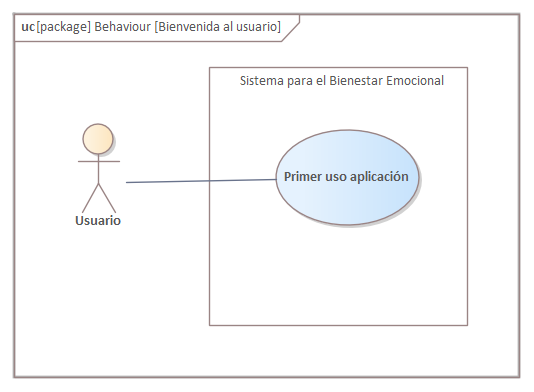
\includegraphics[width=0.75\textwidth]{figures/diseno/casos_uso/Bienvenida al usuario.png}
                \caption{Diagrama de casos de uso de la \textit{feature} \textbf{F-1}}
                \label{figure:diagrama_casos_uso:f1}
            \end{figure}

            Del diagrama anterior únicamente se puede extraer el caso de uso \textbf{CU-1}\phantomsection\label{disenio:casos_uso:primer_uso}: \textit{Primer uso de la aplicación}. La especificación detallada de este caso de uso se encuentra en la Tabla \ref{tabla:casos_uso:primer_uso}; mientras que su diagrama de secuencia se puede encontrar en la Figura \ref{figure:diagrama_secuencia:primer_uso}.

            \begin{table}[h]
                \centering
                \begin{tabularx}{\textwidth}{|l|l|X|}
                    \hline
                    \textbf{ID:} CU-1 & \multicolumn{2}{|X|}{\textbf{Nombre}: Primer uso de la aplicación} \\
                    \hline
                    \textbf{Evento activador} & \multicolumn{2}{|X|}{El usuario abre por primera vez la aplicación} \\
                    \hline
                    \textbf{Actor primario} & \multicolumn{2}{|X|}{Usuario} \\
                    \hline
                    \textbf{Precondición} & \multicolumn{2}{|X|}{El usuario tiene instalado el \gls{framework} Salud Conectada en su dispositivo} \\
                    \hline
                    \multirow{10}{*}{\textbf{Flujo normal}} & \textbf{Paso} & \textbf{Acción} \\
                    \cline{2-3} & 1 & La aplicación presenta al usuario el panel de bienvenida \\
                    \cline{2-3} & 2 & El usuario finaliza u omite el panel de bienvenida \\
                    \cline{2-3} & 3 & La aplicación presenta al usuario una ventana de permisos, solicitando el permiso de notificaciones y de cada tipo de dato de actividad física \\
                    \cline{2-3} & 3.1 & Para cada permiso, la aplicación muestra un botón para otorgar dicho permiso y su motivación \\
                    \cline{2-3} & 4 & El usuario otorga los permisos según sus preferencias \\
                    \cline{2-3} & 5 & El usuario confirma su elección de permisos \\
                    \cline{2-3} & 6 & La aplicación crea los canales de notificación \\
                    \cline{2-3} & 7 & La aplicación planifica las tareas recurrentes \\
                    \cline{2-3} & 8 & La aplicación guarda en la base de datos para cada tipo de dato de actividad física la marca de tiempo actual \\
                    \hline
                    \textbf{Flujo alternativo} & \multicolumn{2}{|X|}{Ninguno} \\
                    \hline
                    \textbf{Postcondición} & \multicolumn{2}{|X|}{El usuario es redirigido a la página principal} \\
                    \hline
                    \textbf{Excepciones} & \multicolumn{2}{|X|}{Ninguna} \\
                    \hline
                \end{tabularx}
                \caption{Especificación del caso de uso \hyperref[disenio:casos_uso:primer_uso]{CU-1}}
                \label{tabla:casos_uso:primer_uso}
            \end{table}  

            \begin{figure}[h]
                \centering
                \includegraphics[width=1\textwidth]{figures/diseno/secuencia/Primer uso aplicación.png}
                \caption{Diagrama de secuencia de \hyperref[disenio:casos_uso:primer_uso]{CU-1}}
                \label{figure:diagrama_secuencia:primer_uso}
            \end{figure}

            \clearpage  % Asegura que todas las figuras y tablas pendientes se impriman antes de continuar.

        \subsection*{Feature 2: Extracción de datos de un dispositivo wearable}

            Esta \textit{feature} describe la funcionalidad asociada a la extracción de datos de un dispositivo \gls{wearable}, permitiendo la aplicación el acceso a los mismos, la visualización de los datos recogidos del usuario por el propio usuario y la visualización de todos los datos recolectados por parte del analista de datos. En la Figura \ref{figure:diagrama_casos_uso:f2} se presenta el diagrama de casos de uso correspondiente.

            \begin{figure}[h]
                \centering
                \includegraphics[width=1\textwidth]{figures/diseno/casos_uso/Extracción datos wearable.png}
                \caption{Diagrama de casos de uso de la \textit{feature} \textbf{F-2}}
                \label{figure:diagrama_casos_uso:f2}
            \end{figure}

            Del diagrama anterior se pueden extraer los siguientes casos de uso:

            \begin{enumerate}[series=casos-uso,label=\textbf{\texttt{CU-\arabic*}}]
                \setcounter{enumi}{1}
                \item \label{disenio:casos_uso:sincronizacion_datos_wearable} Sincronización de los datos del dispositivo \gls{wearable}
                \item \label{disenio:casos_uso:visualizacion_local_wearable} Visualización local de los datos del dispositivo \gls{wearable}
                \item \label{disenio:casos_uso:visualizacion_general_actividad} Visualización general de los datos de actividad física
            \end{enumerate}
            
            La especificación detallada de estos casos de uso se encuentran en la Tablas \ref{tabla:casos_uso:sincronizacion_datos_wearable}, \ref{tabla:casos_uso:visualizacion_local_wearable} y \ref{tabla:casos_uso:visualizacion_general_actividad} respectivamente, mientras que los diagramas de secuencia correspondientes se pueden encontrar en las Figuras \ref{figure:diagrama_secuencia:acceso_datos} \ref{figure:diagrama_secuencia:visualizacion_local_wearable} y \ref{figure:diagrama_secuencia:visualizacion_general_actividad} respectivamente.

            %\todo[inline]{Me sale bajo un mismo caso de uso el acceso, envío y procesado de datos porque de lo contrario me quedan casos de uso sin usuario}
            %\todo[inline]{No tengo claro el \textbf{Evento activador}, si es algo que hace el usuario o viene de un actor implícito como el SO}

            \begin{table}[h]
                \centering
                \begin{tabularx}{\textwidth}{|l|l|X|}
                    \hline
                    \textbf{ID:} CU-2 & \multicolumn{2}{|X|}{\textbf{Nombre}: Sincronización de los datos del dispositivo \gls{wearable}} \\
                    \hline
                    \textbf{Evento activador} & \multicolumn{2}{|X|}{Activación por parte de Android del procedimiento de extracción de datos} \\
                    \hline
                    \textbf{Actor primario} & \multicolumn{2}{|X|}{Usuario} \\
                    \hline
                    \textbf{Precondición} & \multicolumn{2}{|X|}{El usuario dispone de un \gls{wearable}, lo utiliza  y ha completado la fase de bienvenida} \\
                    \hline
                    \multirow{11}{*}{\textbf{Flujo normal}} & \textbf{Paso} & \textbf{Acción} \\
                    \cline{2-3} & 1 & El sistema comprueba si dispone de permisos para al menos un tipo de dato \\
                    \cline{2-3} & 2 & Para cada tipo de dato \\
                    \cline{2-3} & 2.1 & Se comprueba el permiso de lectura \\
                    \cline{2-3} & 2.2 & Si el usuario otorgó el permiso, la aplicación lee los registros del usuario de ese tipo de dato desde la última lectura registrada hasta el instante actual \\
                    \cline{2-3} & 2.3 & Se procesa cada registro leído para mantener únicamente las marcas de tiempo y los datos de la propia medición \\
                    \cline{2-3} & 3 & La aplicación envía al servidor la información recopilada junto al identificador de usuario \\
                    \cline{2-3} & 4 & El servidor comprueba el formato de los datos enviados  \\
                    \cline{2-3} & 5 & El servidor guarda en su base de datos la información recibida \\
                    \cline{2-3} & 6 & El servidor envía, para cada tipo de dato, la marca de tiempo del último registro insertado en base de datos (o nulo si no se ha insertado ningún registro para ese tipo de dato) \\
                    \cline{2-3} & 7 & La aplicación guarda en su base de datos las marcas de tiempo recibidas junto a su tipo de datos \\     
                    \hline
                    \multirow{2}{*}{\textbf{Flujo alternativo}} & \textbf{Paso} & \textbf{Acción} \\
                    \cline{2-3} & 2.2 & Si el usuario no otorgó el permiso, se omite la lectura de ese tipo de dato \\
                    \hline
                    \textbf{Postcondición} & \multicolumn{2}{|X|}{Ninguna} \\
                    \hline
                    \multirow{4}{*}{\textbf{Excepciones}} & \textbf{Paso} & \textbf{Acción} \\
                    \cline{2-3} & 1 & Si la aplicación no dispone de permiso de lectura para ningún tipo de datos, el caso de uso termina \\
                    \cline{2-3} & 3 & Si no se puede enviar correctamente la información, el caso de uso termina \\
                    \cline{2-3} & 4 & Si el formato de los datos enviados es inválido, el servidor envía un código de error y el caso de uso termina \\
                    \hline
                    \caption{Especificación del caso de uso \ref{disenio:casos_uso:sincronizacion_datos_wearable}}
                    \label{tabla:casos_uso:sincronizacion_datos_wearable}
                \end{tabularx}
            \end{table}

            \begin{figure}[h]
                \centering
                \includegraphics[width=1\textwidth]{figures/diseno/secuencia/Sincronización datos wearable.png}
                \caption{Diagrama de secuencia de \ref{disenio:casos_uso:sincronizacion_datos_wearable}}
                \label{figure:diagrama_secuencia:acceso_datos}
            \end{figure}
            
            \begin{table}[h]
                \centering
                \begin{tabularx}{\textwidth}{|l|l|X|}
                    \hline
                    \textbf{ID:} CU-3 & \multicolumn{2}{|X|}{\textbf{Nombre}: Visualización local de los datos del \gls{wearable}} \\
                    \hline
                    \textbf{Evento activador} & \multicolumn{2}{|X|}{El usuario ha indicado visualizar sus datos del \gls{wearable}} \\
                    \hline
                    \textbf{Actor primario} & \multicolumn{2}{|X|}{Usuario} \\
                    \hline
                    \textbf{Precondición} & \multicolumn{2}{|X|}{El usuario ha completado la fase de bienvenida} \\
                    \hline
                    \multirow{7}{*}{\textbf{Flujo normal}} & \textbf{Paso} & \textbf{Acción} \\
                    \cline{2-3} & 1 & La aplicación dispone al usuario un panel con cada uno de los tipos de datos disponibles \\
                    \cline{2-3} & 2 & El usuario pulsa sobre el tipo de datos que quiere visualizar \\
                    \cline{2-3} & 3 & La aplicación comprueba si dispone de permiso de lectura  \\
                    \cline{2-3} & 4 & La aplicación lee todos los datos recopilados sobre ese tipo de datos \\
                    \cline{2-3} & 5 & La aplicación procesa cada registro para dotarle de interfaz gráfica \\
                    \cline{2-3} & 6 & La aplicación muestra los datos procesados \\
                    \cline{2-3} & 7 & El usuario visualiza los datos hasta que bien o pulsa sobre otro tipo de dato o sale de la ventana finalizando el caso de uso \\
                    \hline
                    \multirow{6}{*}{\textbf{Flujo alternativo}} & \textbf{Paso} & \textbf{Acción} \\
                    \cline{2-3} & 3 & Si la aplicación no dispone de permiso de lectura, se mostrará un botón para que el usuario pueda otorgarlo \\
                    \cline{2-3} & 3.1 & Si el usuario otorga el permiso de lectura, se retoma el flujo normal en el paso 4 \\
                    \cline{2-3} & 3.2 & Si el usuario no otorga el permiso de lectura, se finaliza el caso de uso \\
                    \cline{2-3} & 4 & Si no hay datos recopilados, la aplicación mostrará un mensaje indicando la ausencia de datos, retomándose el flujo normal en el paso 7 \\
                    \cline{2-3} & 7 & Si el usuario pulsa sobre otro tipo de dato, se retoma el flujo normal en el paso 3 \\
                    \hline
                    \textbf{Postcondición} & \multicolumn{2}{|X|}{Ninguna} \\
                    \hline
                    \textbf{Excepciones} & \multicolumn{2}{|X|}{Ninguna} \\
                    \hline
                    \caption{Especificación del caso de uso \ref{disenio:casos_uso:visualizacion_local_wearable}}
                    \label{tabla:casos_uso:visualizacion_local_wearable}
                \end{tabularx}
            \end{table}

            \begin{figure}[h]
                \centering
                \includegraphics[width=1\textwidth]{figures/diseno/secuencia/Visualización datos wearable.png}
                \caption{Diagrama de secuencia de \ref{disenio:casos_uso:visualizacion_local_wearable}}
                \label{figure:diagrama_secuencia:visualizacion_local_wearable}
            \end{figure}
            
            \begin{table}[h]
                \centering
                \begin{tabularx}{\textwidth}{|l|l|X|}
                    \hline
                    \textbf{ID:} CU-4 & \multicolumn{2}{|X|}{\textbf{Nombre}: Visualización general de los datos de actividad física} \\
                    \hline
                    \textbf{Evento activador} & \multicolumn{2}{|X|}{El analista de datos ha indicado visualizar los datos generales de actividad física} \\
                    \hline
                    \textbf{Actor primario} & \multicolumn{2}{|X|}{Analista de datos} \\
                    \hline
                    \textbf{Precondición} & \multicolumn{2}{|X|}{Ninguna} \\
                    \hline
                    \multirow{3}{*}{\textbf{Flujo normal}} & \textbf{Paso} & \textbf{Acción} \\
                    \cline{2-3} & 1 & El analista de datos se conecta a la base de datos del servidor \\
                    \cline{2-3} & 2 & El analista de datos puede consultar para cada identificador de usuario, los datos de actividad física \\
                    \hline
                    \textbf{Flujo alternativo} & \multicolumn{2}{|X|}{Ninguno} \\
                    \hline
                    \textbf{Postcondición} & \multicolumn{2}{|X|}{Ninguna} \\
                    \hline
                    \textbf{Excepciones} & \multicolumn{2}{|X|}{Ninguna} \\
                    \hline
                    \caption{Especificación del caso de uso \ref{disenio:casos_uso:visualizacion_general_actividad}}
                    \label{tabla:casos_uso:visualizacion_general_actividad}
                \end{tabularx}
            \end{table}
    
            \begin{figure}[h]
                \centering
                \includegraphics[width=0.75\textwidth]{figures/diseno/secuencia/Visualización general datos actividad fisica.png}
                \caption{Diagrama de secuencia de \ref{disenio:casos_uso:visualizacion_general_actividad}}
                \label{figure:diagrama_secuencia:visualizacion_general_actividad}
            \end{figure}

        \clearpage  % Asegura que todas las figuras y tablas pendientes se impriman antes de continuar.

        \subsection*{Feature 3: Seguimiento individual}

            Esta característica describe todas las acciones que el usuario puede realizar acerca del seguimiento individual de las diferentes enfermedades. Por una parte el sistema realizará el seguimiento del estrés, depresión y riesgo de suicidio, implementará el cuestionario de contraste y permitirá visualizar los niveles de estrés, soledad y depresión. 
            
            El diagrama de casos de uso de esta \textit{feature} se puede encontrar en la Figura \ref{figure:diagrama_casos_uso:f3}.

            \begin{figure}[h]
                \centering
                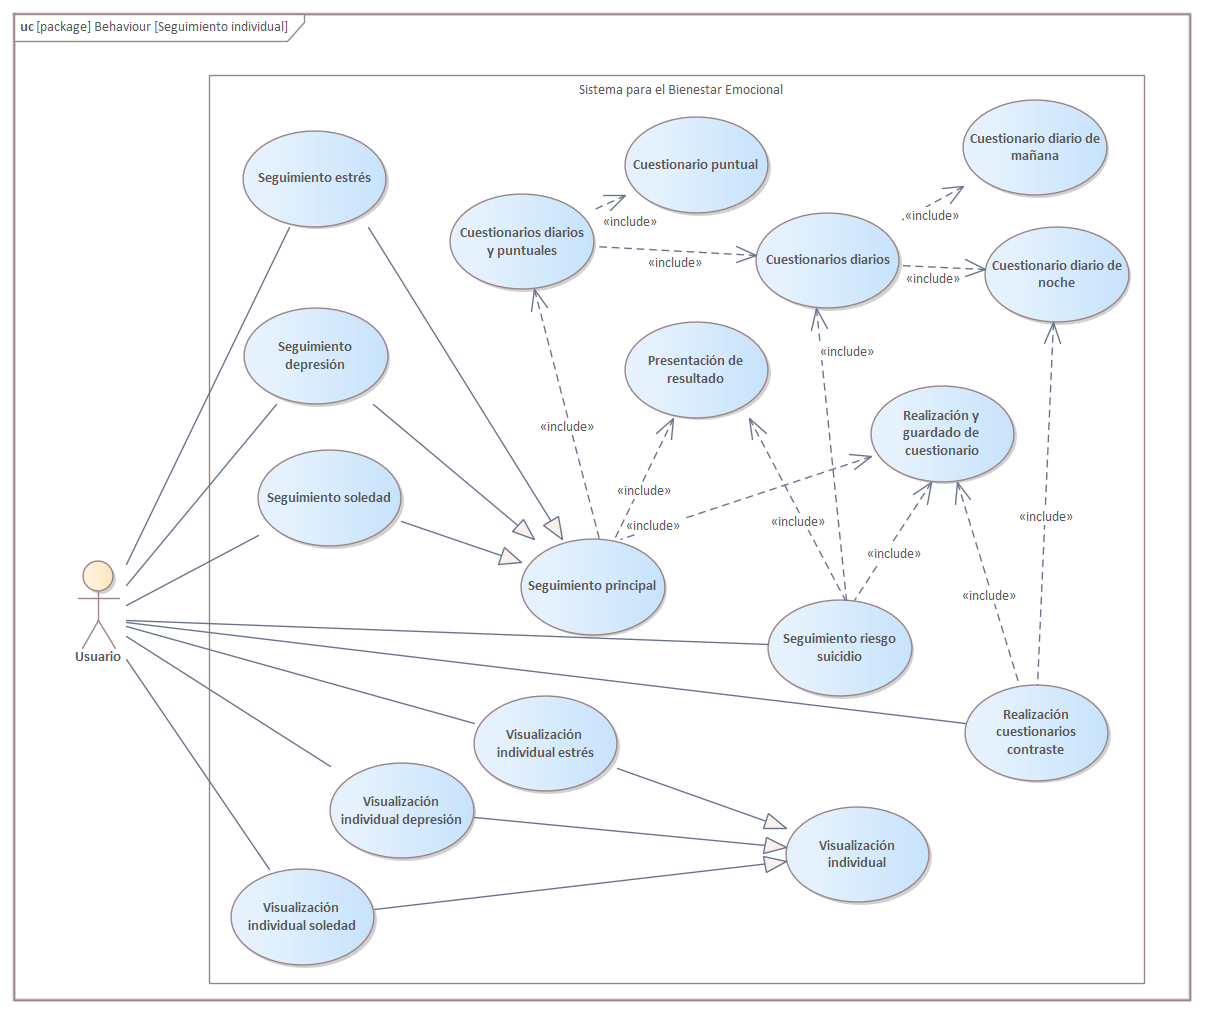
\includegraphics[width=1\textwidth]{figures/diseno/casos_uso/Seguimiento individual.png}
                \caption{Diagrama de casos de uso de la \textit{feature} \textbf{F-3}}
                \label{figure:diagrama_casos_uso:f3}
            \end{figure}

            A diferencia de las \textit{features} anteriores, esta consta de mayor complejidad, ya que según la enfermedad en cuestión aplican unas frecuencias de cuestionarios diferentes o se varía la necesidad de presentar de resultados.

            Del diagrama anterior los casos de uso asociados con el usuario son, a saber:

            \begin{enumerate}[resume=casos-uso,label=\textbf{\texttt{CU-\arabic*}}]
                \item \label{disenio:casos_uso:seguimiento_estres} Seguimiento del estrés
                \item \label{disenio:casos_uso:seguimiento_depresion} Seguimiento de la depresión
                \item \label{disenio:casos_uso:seguimiento_suicidio} Seguimiento del riesgo de suicidio
                \item \label{disenio:casos_uso:seguimiento_soledad} Seguimiento de la soledad
                \item \label{disenio:casos_uso:cuestionarios_contraste} Realización de los cuestionarios contraste
                \item \label{disenio:casos_uso:visualizacion_individual_estres} Visualización individual del estrés
                \item \label{disenio:casos_uso:visualizacion_individual_depresion} Visualización individual de la depresión
                \item \label{disenio:casos_uso:visualizacion_individual_soledad} Visualización individual de la soledad
            \end{enumerate}

            La especificación detallada de estos casos de uso se encuentran en la Tablas \ref{tabla:casos_uso:seguimiento_estres}, \ref{tabla:casos_uso:seguimiento_depresion}, \ref{tabla:casos_uso:seguimiento_suicidio}, \ref{tabla:casos_uso:seguimiento_soledad}, \ref{tabla:casos_uso:cuestionarios_contraste}, \ref{tabla:casos_uso:visualizacion_individual_estres},
            \ref{tabla:casos_uso:visualizacion_individual_depresion} y  \ref{tabla:casos_uso:visualizacion_individual_soledad} respectivamente. 

            A diferencia de los casos anteriores, los diagramas de secuencia propuestos no hacen referencia a los casos de uso que interactúan con el usuario sino con los abstractos. Mediante el modelado de estos casos de uso se permite generalizar flujos de eventos del sistema, logrando mejorar la legibilidad del proceso de modelado.

            En particular, las Figuras \ref{figure:diagrama_secuencia:realizacion_guardado_cuestionario}, \ref{figure:diagrama_secuencia:presentacion_resultado}, \ref{figure:diagrama_secuencia:visualizacion_individual} hacen referencia a los casos de uso \textit{Realización y guardado de cuestionario}, \textit{Presentación de resultado} y \textit{Visualización individual} respectivamente.

            \begin{table}[h]
                \centering
                \begin{tabularx}{\textwidth}{|l|l|X|}
                    \hline
                    \textbf{ID:} CU-5 & \multicolumn{2}{|X|}{\textbf{Nombre}: Seguimiento del estrés} \\
                    \hline
                    \textbf{Evento activador} & \multicolumn{2}{|X|}{Activación por parte de Android del procedimiento de seguimiento del estrés} \\
                    \hline
                    \textbf{Actor primario} & \multicolumn{2}{|X|}{Usuario} \\
                    \hline
                    \textbf{Precondición} & \multicolumn{2}{|X|}{El usuario ha completado la fase de bienvenida} \\
                    \hline
                    \multirow{13}{*}{\textbf{Flujo normal}} & \textbf{Paso} & \textbf{Acción} \\
                    \cline{2-3} & 1 & La aplicación crea uno de los siguientes tres cuestionarios \\
                    \cline{2-3} & 1.1 & Diario matutino \\
                    \cline{2-3} & 1.2 & Diario vespertino \\
                    \cline{2-3} & 1.3 & Puntual \\
                    \cline{2-3} & 2 & La aplicación crea una notificación al usuario \\
                    \cline{2-3} & 3 & El usuario pulsa en la notificación \\
                    \cline{2-3} & 4 & La aplicación muestra al usuario el cuestionario \\
                    \cline{2-3} & 5 & El usuario rellena el cuestionario \\
                    \cline{2-3} & 6 & El usuario finaliza el cuestionario \\
                    \cline{2-3} & 7 & La aplicación computa el cuestionario, obteniendo su puntuación numérica del cuestionario, el nivel cualitativo de estrés según el cuestionario y un consejo acorde al nivel \\
                    \cline{2-3} & 8 & La aplicación muestra al usuario la puntuación numérica del cuestionario, el nivel cualitativo según el cuestionario y un consejo acorde al nivel \\
                    \cline{2-3} & 9 & El cuestionario se guarda en base de datos \\
                    \hline
                    \multirow{6}{*}{\textbf{Flujo alternativo}} & \textbf{Paso} & \textbf{Acción} \\
                    \cline{2-3} & 5 & El usuario omite la finalización del cuestionario \\
                    \cline{2-3} & 5.1 & Se guarda en base de datos la información disponible del cuestionario \\
                    \cline{2-3} & 5.2 & Cuando el usuario visite la página principal, se mostrará un aviso de cuestionarios incompletos para que el usuario pueda retomarlo, reanudándose el flujo normal en el paso 4 \\
                    \cline{2-3} & 6 & El usuario no ha respondido a todas las preguntas \\
                    \cline{2-3} & 6.1 & La aplicación muestra al usuario las preguntas restantes, reanudándose el flujo normal en el paso 5 \\
                    \hline
                    \textbf{Postcondición} & \multicolumn{2}{|X|}{La aplicación devuelve al usuario a la página principal} \\
                    \hline
                    \multirow{2}{*}{\textbf{Excepciones}}  & \textbf{Paso} & \textbf{Acción} \\
                    \cline{2-3} & 2 & Si el usuario no ha indicado el permiso de notificaciones, el usuario podrá abrir el cuestionario mediante el aviso de cuestionarios incompletos de la página principal \\
                    \hline
                    \caption{Especificación del caso de uso \ref{disenio:casos_uso:seguimiento_estres}}
                    \label{tabla:casos_uso:seguimiento_estres}
                \end{tabularx}
            \end{table}

            \begin{table}[h]
                \centering
                \begin{tabularx}{\textwidth}{|l|l|X|}
                    \hline
                    \textbf{ID:} CU-6 & \multicolumn{2}{|X|}{\textbf{Nombre}: Seguimiento de la depresión} \\
                    \hline
                    \textbf{Evento activador} & \multicolumn{2}{|X|}{Activación por parte de Android del procedimiento de seguimiento de la depresión} \\
                    \hline
                    \textbf{Actor primario} & \multicolumn{2}{|X|}{Usuario} \\
                    \hline
                    \textbf{Precondición} & \multicolumn{2}{|X|}{El usuario ha completado la fase de bienvenida y ha permitido la monitorización de la depresión} \\
                    \hline
                    \multirow{13}{*}{\textbf{Flujo normal}} & \textbf{Paso} & \textbf{Acción} \\
                    \cline{2-3} & 1 & La aplicación crea uno de los siguientes tres cuestionarios \\
                    \cline{2-3} & 1.1 & Diario matutino \\
                    \cline{2-3} & 1.2 & Diario vespertino \\
                    \cline{2-3} & 1.3 & Puntual \\
                    \cline{2-3} & 2 & La aplicación crea una notificación al usuario \\
                    \cline{2-3} & 3 & El usuario pulsa en la notificación \\
                    \cline{2-3} & 4 & La aplicación muestra al usuario el cuestionario \\
                    \cline{2-3} & 5 & El usuario rellena el cuestionario \\
                    \cline{2-3} & 6 & El usuario finaliza el cuestionario \\
                    \cline{2-3} & 7 & La aplicación computa el cuestionario, obteniendo su puntuación numérica del cuestionario, el nivel cualitativo de depresión según el cuestionario y un consejo acorde al nivel \\
                    \cline{2-3} & 8 & La aplicación muestra al usuario la puntuación numérica del cuestionario, el nivel cualitativo según el cuestionario y un consejo acorde al nivel \\
                    \cline{2-3} & 9 & El cuestionario se guarda en base de datos \\
                    \hline
                    \multirow{6}{*}{\textbf{Flujo alternativo}} & \textbf{Paso} & \textbf{Acción} \\
                    \cline{2-3} & 5 & El usuario omite la finalización del cuestionario \\
                    \cline{2-3} & 5.1 & Se guarda en base de datos la información disponible del cuestionario \\
                    \cline{2-3} & 5.2 & Cuando el usuario visite la página principal, se mostrará un aviso de cuestionarios incompletos para que el usuario pueda retomarlo, reanudándose el flujo normal en el paso 4 \\
                    \cline{2-3} & 6 & El usuario no ha respondido a todas las preguntas \\
                    \cline{2-3} & 6.1 & La aplicación muestra al usuario las preguntas restantes, reanudándose el flujo normal en el paso 5 \\
                    \hline
                    \textbf{Postcondición} & \multicolumn{2}{|X|}{La aplicación devuelve al usuario a la página principal} \\
                    \hline
                    \multirow{2}{*}{\textbf{Excepciones}}  & \textbf{Paso} & \textbf{Acción} \\
                    \cline{2-3} & 2 & Si el usuario no ha indicado el permiso de notificaciones, el usuario podrá abrir el cuestionario mediante el aviso de cuestionarios incompletos de la página principal \\
                    \hline
                    \caption{Especificación del caso de uso \ref{disenio:casos_uso:seguimiento_depresion}}
                    \label{tabla:casos_uso:seguimiento_depresion}
                \end{tabularx}
            \end{table}

            \begin{table}[h]
                \centering
                \begin{tabularx}{\textwidth}{|l|l|X|}
                    \hline
                    \textbf{ID:} CU-7 & \multicolumn{2}{|X|}{\textbf{Nombre}: Seguimiento del riesgo de suicidio} \\
                    \hline
                    \textbf{Evento activador} & \multicolumn{2}{|X|}{Activación por parte de Android del procedimiento de seguimiento del riesgo de suicidio} \\
                    \hline
                    \textbf{Actor primario} & \multicolumn{2}{|X|}{Usuario} \\
                    \hline
                    \textbf{Precondición} & \multicolumn{2}{|X|}{El usuario ha completado la fase de bienvenida y ha permitido la monitorización de la depresión} \\
                    \hline
                    \multirow{11}{*}{\textbf{Flujo normal}} & \textbf{Paso} & \textbf{Acción} \\
                    \cline{2-3} & 1 & La aplicación crea uno de los siguientes dos cuestionarios \\
                    \cline{2-3} & 1.1 & Diario matutino \\
                    \cline{2-3} & 1.2 & Diario vespertino \\
                    \cline{2-3} & 2 & La aplicación crea una notificación al usuario \\
                    \cline{2-3} & 3 & El usuario pulsa en la notificación \\
                    \cline{2-3} & 4 & La aplicación muestra al usuario el cuestionario \\
                    \cline{2-3} & 5 & El usuario rellena el cuestionario \\
                    \cline{2-3} & 6 & El usuario finaliza el cuestionario \\
                    \cline{2-3} & 7 & La aplicación computa el cuestionario, obteniendo el nivel de riesgo de suicidio y un consejo acorde al nivel \\
                    \cline{2-3} & 8 & La aplicación muestra al usuario un consejo acorde al nivel de riesgo e suicidio \\
                    \cline{2-3} & 9 & El cuestionario se guarda en base de datos \\
                    \hline
                    \multirow{6}{*}{\textbf{Flujo alternativo}} & \textbf{Paso} & \textbf{Acción} \\
                    \cline{2-3} & 5 & El usuario omite la finalización del cuestionario \\
                    \cline{2-3} & 5.1 & Se guarda en base de datos la información disponible del cuestionario \\
                    \cline{2-3} & 5.2 & Cuando el usuario visite la página principal, se mostrará un aviso de cuestionarios incompletos para que el usuario pueda retomarlo, reanudándose el flujo normal en el paso 4 \\
                    \cline{2-3} & 6 & El usuario no ha respondido a todas las preguntas \\
                    \cline{2-3} & 6.1 & La aplicación muestra al usuario las preguntas restantes, reanudándose el flujo normal en el paso 5 \\
                    \hline
                    \textbf{Postcondición} & \multicolumn{2}{|X|}{La aplicación devuelve al usuario a la página rincipal} \\
                    \hline
                    \multirow{2}{*}{\textbf{Excepciones}}  & \textbf{Paso} & \textbf{Acción} \\
                    \cline{2-3} & 2 & Si el usuario no ha indicado el permiso de notificaciones, el usuario podrá abrir el cuestionario mediante el aviso de cuestionarios incompletos de la página principal \\
                    \hline
                    \caption{Especificación del caso de uso \ref{disenio:casos_uso:seguimiento_suicidio}}
                    \label{tabla:casos_uso:seguimiento_suicidio}
                \end{tabularx}
            \end{table}

            \begin{table}[h]
                \centering
                \begin{tabularx}{\textwidth}{|l|l|X|}
                    \hline
                    \textbf{ID:} CU-8 & \multicolumn{2}{|X|}{\textbf{Nombre}: Seguimiento de la soledad} \\
                    \hline
                    \textbf{Evento activador} & \multicolumn{2}{|X|}{Activación por parte de Android del procedimiento de seguimiento de la soledad} \\
                    \hline
                    \textbf{Actor primario} & \multicolumn{2}{|X|}{Usuario} \\
                    \hline
                    \textbf{Precondición} & \multicolumn{2}{|X|}{El usuario ha completado la fase de bienvenida y ha permitido la monitorización de la soledad} \\
                    \hline
                    \multirow{13}{*}{\textbf{Flujo normal}} & \textbf{Paso} & \textbf{Acción} \\
                    \cline{2-3} & 1 & La aplicación crea uno de los siguientes tres cuestionarios \\
                    \cline{2-3} & 1.1 & Diario matutino \\
                    \cline{2-3} & 1.2 & Diario vespertino \\
                    \cline{2-3} & 1.3 & Puntual \\
                    \cline{2-3} & 2 & La aplicación crea una notificación al usuario \\
                    \cline{2-3} & 3 & El usuario pulsa en la notificación \\
                    \cline{2-3} & 4 & La aplicación muestra al usuario el cuestionario \\
                    \cline{2-3} & 5 & El usuario rellena el cuestionario \\
                    \cline{2-3} & 6 & El usuario finaliza el cuestionario \\
                    \cline{2-3} & 7 & La aplicación computa el cuestionario, obteniendo su puntuación numérica del cuestionario, el nivel cualitativo de soledad según el cuestionario y un consejo acorde al nivel \\
                    \cline{2-3} & 8 & La aplicación muestra al usuario la puntuación numérica del cuestionario, el nivel cualitativo según el cuestionario y un consejo acorde al nivel \\
                    \cline{2-3} & 9 & El cuestionario se guarda en base de datos \\
                    \hline
                    \multirow{6}{*}{\textbf{Flujo alternativo}} & \textbf{Paso} & \textbf{Acción} \\
                    \cline{2-3} & 5 & El usuario omite la finalización del cuestionario \\
                    \cline{2-3} & 5.1 & Se guarda en base de datos la información disponible del cuestionario \\
                    \cline{2-3} & 5.2 & Cuando el usuario visite la página principal, se mostrará un aviso de cuestionarios incompletos para que el usuario pueda retomarlo, reanudándose el flujo normal en el paso 4 \\
                    \cline{2-3} & 6 & El usuario no ha respondido a todas las preguntas \\
                    \cline{2-3} & 6.1 & La aplicación muestra al usuario las preguntas restantes, reanudándose el flujo normal en el paso 5 \\
                    \hline
                    \textbf{Postcondición} & \multicolumn{2}{|X|}{La aplicación devuelve al usuario a la página principal} \\
                    \hline
                    \multirow{2}{*}{\textbf{Excepciones}}  & \textbf{Paso} & \textbf{Acción} \\
                    \cline{2-3} & 2 & Si el usuario no ha indicado el permiso de notificaciones, el usuario podrá abrir el cuestionario mediante el aviso de cuestionarios incompletos de la página principal \\
                    \hline
                    \caption{Especificación del caso de uso \ref{disenio:casos_uso:seguimiento_soledad}}
                    \label{tabla:casos_uso:seguimiento_soledad}
                \end{tabularx}
            \end{table}

            \begin{table}[h]
                \centering
                \begin{tabularx}{\textwidth}{|l|l|X|}
                    \hline
                    \textbf{ID:} CU-9 & \multicolumn{2}{|X|}{\textbf{Nombre}: Realización de los cuestionarios contraste} \\
                    \hline
                    \textbf{Evento activador} & \multicolumn{2}{|X|}{Activación por parte de Android del procedimiento de cuestionarios contraste} \\
                    \hline
                    \textbf{Actor primario} & \multicolumn{2}{|X|}{Usuario} \\
                    \hline
                    \textbf{Precondición} & \multicolumn{2}{|X|}{El usuario ha completado la fase de bienvenida} \\
                    \hline
                    \multirow{8}{*}{\textbf{Flujo normal}} & \textbf{Paso} & \textbf{Acción} \\
                    \cline{2-3} & 1 & La aplicación crea el cuestionario diariamente en horario vespertino \\
                    \cline{2-3} & 2 & La aplicación crea una notificación al usuario \\
                    \cline{2-3} & 3 & El usuario pulsa en la notificación \\
                    \cline{2-3} & 4 & La aplicación muestra al usuario el cuestionario \\
                    \cline{2-3} & 5 & El usuario rellena el cuestionario \\
                    \cline{2-3} & 6 & El usuario finaliza el cuestionario \\
                    \cline{2-3} & 7 & El cuestionario se guarda en base de datos \\
                    \hline
                    \multirow{6}{*}{\textbf{Flujo alternativo}} & \textbf{Paso} & \textbf{Acción} \\
                    \cline{2-3} & 5 & El usuario omite la finalización del cuestionario \\
                    \cline{2-3} & 5.1 & Se guarda en base de datos la información disponible del cuestionario \\
                    \cline{2-3} & 5.2 & Cuando el usuario visite la página principal, se mostrará un aviso de cuestionarios incompletos para que el usuario pueda retomarlo, reanudándose el flujo normal en el paso 4 \\
                    \cline{2-3} & 6 & El usuario no ha respondido a todas las preguntas \\
                    \cline{2-3} & 6.1 & La aplicación muestra al usuario las preguntas restantes, reanudándose el flujo normal en el paso 5 \\
                    \hline
                    \textbf{Postcondición} & \multicolumn{2}{|X|}{La aplicación devuelve al usuario a la página principal} \\
                    \hline
                    \multirow{2}{*}{\textbf{Excepciones}}  & \textbf{Paso} & \textbf{Acción} \\
                    \cline{2-3} & 2 & Si el usuario no ha indicado el permiso de notificaciones, el usuario podrá abrir el cuestionario mediante el aviso de cuestionarios incompletos de la página principal \\
                    \hline
                    \caption{Especificación del caso de uso \ref{disenio:casos_uso:cuestionarios_contraste}}
                    \label{tabla:casos_uso:cuestionarios_contraste}
                \end{tabularx}
            \end{table}

            \begin{table}[h]
                \centering
                \begin{tabularx}{\textwidth}{|l|l|X|}
                    \hline
                    \textbf{ID:} CU-10 & \multicolumn{2}{|X|}{\textbf{Nombre}: Visualización individual del estrés} \\
                    \hline
                    \textbf{Evento activador} & \multicolumn{2}{|X|}{El usuario accede a la ventana principal de la aplicación} \\
                    \hline
                    \textbf{Actor primario} & \multicolumn{2}{|X|}{Usuario} \\
                    \hline
                    \textbf{Precondición} & \multicolumn{2}{|X|}{El usuario ha completado la fase de bienvenida} \\
                    \hline
                    \multirow{13}{*}{\textbf{Flujo normal}} & \textbf{Paso} & \textbf{Acción} \\
                    \cline{2-3} & 1 & La aplicación accede al último cuestionario de estrés \\
                    \cline{2-3} & 2 & La aplicación muestra la puntuación de dicho cuestionario, el nivel cualitativo, un consejo sobre el mismo y un botón para el acceso a estadísticas más detalladas \\
                    \cline{2-3} & 3 & El usuario visualiza los datos \\
                    \cline{2-3} & 4 & El usuario pulsa en el botón de estadísticas más detalladas \\
                    \cline{2-3} & 5.1 & La aplicación accede a los resultados de los cuestionarios de estrés del día anterior \\
                    \cline{2-3} & 5.2 & La aplicación accede a los resultados de los cuestionarios de estrés de los últimos siete días \\
                    \cline{2-3} & 5.3 & La aplicación accede a los resultados de los cuestionarios de estrés de la semana actual \\
                    \cline{2-3} & 6.1 & La aplicación computará la media de las puntuaciones de los cuestionarios de estrés del día anterior y el nivel cualitativo correspondiente \\
                    \cline{2-3} & 6.2 & La aplicación computará la media de las puntuaciones de los cuestionarios de estrés de los últimos siete días y el nivel cualitativo correspondiente \\
                    \cline{2-3} & 6.3 & La aplicación computará, para cada día de la semana actual, la media de las puntuaciones de los cuestionarios de estrés \\
                    \cline{2-3} & 7 & La aplicación mostrará los datos computados en el paso anterior, junto con un botón para visualizar estadísticas más detalladas \\
                    \cline{2-3} & 8 & El usuario visualiza los datos hasta que sale de la ventana finalizando el caso de uso \\
                    \hline
                    \multirow{4}{*}{\textbf{Flujo alternativo}} & \textbf{Paso} & \textbf{Acción} \\
                    \cline{2-3} & 2 & Si el último cuestionario de estrés no ha sido finalizado, se mostrará una puntuación y nivel nulos \\
                    \cline{2-3} & 4 & El usuario finaliza la visualización de los datos saliendo de la ventana. Se termina el caso de uso \\
                    \cline{2-3} & 8 & El usuario pulsa en el botón de estadísticas más detalladas, siendo redirigido a la ventana de historial \\
                    \hline
                    \textbf{Postcondición} & \multicolumn{2}{|X|}{Ninguna} \\
                    \hline
                    \multirow{4}{*}{\textbf{Excepciones}}  & \textbf{Paso} & \textbf{Acción} \\
                    \cline{2-3} & 6.1 & Si no hay puntuaciones de los cuestionarios de estrés del día anterior, se asumirá media y nivel nulos \\
                    \cline{2-3} & 6.2 & Si no hay puntuaciones de los cuestionarios de estrés de los últimos siete días, se asumirá media y nivel nulos \\
                    \cline{2-3} & 6.3 & Si no hay puntuaciones de los cuestionarios de estrés de la semana actual, se asumirá media nula \\
                    \hline
                    \caption{Especificación del caso de uso \ref{disenio:casos_uso:visualizacion_individual_estres}}
                    \label{tabla:casos_uso:visualizacion_individual_estres}
                \end{tabularx}
            \end{table}

            \begin{table}[h]
                \centering
                \begin{tabularx}{\textwidth}{|l|l|X|}
                    \hline
                    \textbf{ID:} CU-11 & \multicolumn{2}{|X|}{\textbf{Nombre}: Visualización individual de la depresión} \\
                    \hline
                    \textbf{Evento activador} & \multicolumn{2}{|X|}{El usuario accede a la ventana principal de la aplicación} \\
                    \hline
                    \textbf{Actor primario} & \multicolumn{2}{|X|}{Usuario} \\
                    \hline
                    \textbf{Precondición} & \multicolumn{2}{|X|}{El usuario ha completado la fase de bienvenida y ha permitido la monitorización de la depresión} \\
                    \hline
                    \multirow{13}{*}{\textbf{Flujo normal}} & \textbf{Paso} & \textbf{Acción} \\
                    \cline{2-3} & 1 & La aplicación accede al último cuestionario de depresión \\
                    \cline{2-3} & 2 & La aplicación muestra la puntuación de dicho cuestionario, el nivel cualitativo, un consejo sobre el mismo y un botón para el acceso a estadísticas más detalladas \\
                    \cline{2-3} & 3 & El usuario visualiza los datos \\
                    \cline{2-3} & 4 & El usuario pulsa en el botón de estadísticas más detalladas \\
                    \cline{2-3} & 5.1 & La aplicación accede a los resultados de los cuestionarios de depresión del día anterior \\
                    \cline{2-3} & 5.2 & La aplicación accede a los resultados de los cuestionarios de depresión de los últimos siete días \\
                    \cline{2-3} & 5.3 & La aplicación accede a los resultados de los cuestionarios de depresión de la semana actual \\
                    \cline{2-3} & 6.1 & La aplicación computará la media de las puntuaciones de los cuestionarios de depresión del día anterior y el nivel cualitativo correspondiente \\
                    \cline{2-3} & 6.2 & La aplicación computará la media de las puntuaciones de los cuestionarios de depresión de los últimos siete días y el nivel cualitativo correspondiente \\
                    \cline{2-3} & 6.3 & La aplicación computará, para cada día de la semana actual, la media de las puntuaciones de los cuestionarios de depresión \\
                    \cline{2-3} & 7 & La aplicación mostrará los datos computados en el paso anterior, junto con un botón para visualizar estadísticas más detalladas \\
                    \cline{2-3} & 8 & El usuario visualiza los datos hasta que sale de la ventana finalizando el caso de uso \\
                    \hline
                    \multirow{4}{*}{\textbf{Flujo alternativo}} & \textbf{Paso} & \textbf{Acción} \\
                    \cline{2-3} & 2 & Si el último cuestionario de depresión no ha sido finalizado, se mostrará una puntuación y nivel nulos \\
                    \cline{2-3} & 4 & El usuario finaliza la visualización de los datos saliendo de la ventana. Se termina el caso de uso \\
                    \cline{2-3} & 8 & El usuario pulsa en el botón de estadísticas más detalladas, siendo redirigido a la ventana de historial \\
                    \hline
                    \textbf{Postcondición} & \multicolumn{2}{|X|}{Ninguna} \\
                    \hline
                    \multirow{4}{*}{\textbf{Excepciones}}  & \textbf{Paso} & \textbf{Acción} \\
                    \cline{2-3} & 6.1 & Si no hay puntuaciones de los cuestionarios de depresión del día anterior, se asumirá media y nivel nulos \\
                    \cline{2-3} & 6.2 & Si no hay puntuaciones de los cuestionarios de depresión de los últimos siete días, se asumirá media y nivel nulos \\
                    \cline{2-3} & 6.3 & Si no hay puntuaciones de los cuestionarios de depresión de la semana actual, se asumirá media nula \\
                    \hline
                    \caption{Especificación del caso de uso \ref{disenio:casos_uso:visualizacion_individual_depresion}}
                    \label{tabla:casos_uso:visualizacion_individual_depresion}
                \end{tabularx}
            \end{table}

            \begin{table}[h]
                \centering
                \begin{tabularx}{\textwidth}{|l|l|X|}
                    \hline
                    \textbf{ID:} CU-12 & \multicolumn{2}{|X|}{\textbf{Nombre}: Visualización individual de la soledad} \\
                    \hline
                    \textbf{Evento activador} & \multicolumn{2}{|X|}{El usuario accede a la ventana principal de la aplicación} \\
                    \hline
                    \textbf{Actor primario} & \multicolumn{2}{|X|}{Usuario} \\
                    \hline
                    \textbf{Precondición} & \multicolumn{2}{|X|}{El usuario ha completado la fase de bienvenida y ha permitido la monitorización de la soledad} \\
                    \hline
                    \multirow{13}{*}{\textbf{Flujo normal}} & \textbf{Paso} & \textbf{Acción} \\
                    \cline{2-3} & 1 & La aplicación accede al último cuestionario de soledad \\
                    \cline{2-3} & 2 & La aplicación muestra la puntuación de dicho cuestionario, el nivel cualitativo, un consejo sobre el mismo y un botón para el acceso a estadísticas más detalladas \\
                    \cline{2-3} & 3 & El usuario visualiza los datos \\
                    \cline{2-3} & 4 & El usuario pulsa en el botón de estadísticas más detalladas \\
                    \cline{2-3} & 5.1 & La aplicación accede a los resultados de los cuestionarios de soledad del día anterior \\
                    \cline{2-3} & 5.2 & La aplicación accede a los resultados de los cuestionarios de soledad de los últimos siete días \\
                    \cline{2-3} & 5.3 & La aplicación accede a los resultados de los cuestionarios de soledad de la semana actual \\
                    \cline{2-3} & 6.1 & La aplicación computará la media de las puntuaciones de los cuestionarios de soledad del día anterior y el nivel cualitativo correspondiente \\
                    \cline{2-3} & 6.2 & La aplicación computará la media de las puntuaciones de los cuestionarios de soledad de los últimos siete días y el nivel cualitativo correspondiente \\
                    \cline{2-3} & 6.3 & La aplicación computará, para cada día de la semana actual, la media de las puntuaciones de los cuestionarios de soledad \\
                    \cline{2-3} & 7 & La aplicación mostrará los datos computados en el paso anterior, junto con un botón para visualizar estadísticas más detalladas \\
                    \cline{2-3} & 8 & El usuario visualiza los datos hasta que sale de la ventana finalizando el caso de uso \\
                    \hline
                    \multirow{4}{*}{\textbf{Flujo alternativo}} & \textbf{Paso} & \textbf{Acción} \\
                    \cline{2-3} & 2 & Si el último cuestionario de soledad no ha sido finalizado, se mostrará una puntuación y nivel nulos \\
                    \cline{2-3} & 4 & El usuario finaliza la visualización de los datos saliendo de la ventana. Se termina el caso de uso \\
                    \cline{2-3} & 8 & El usuario pulsa en el botón de estadísticas más detalladas, siendo redirigido a la ventana de historial \\
                    \hline
                    \textbf{Postcondición} & \multicolumn{2}{|X|}{Ninguna} \\
                    \hline
                    \multirow{4}{*}{\textbf{Excepciones}}  & \textbf{Paso} & \textbf{Acción} \\
                    \cline{2-3} & 6.1 & Si no hay puntuaciones de los cuestionarios de soledad del día anterior, se asumirá media y nivel nulos \\
                    \cline{2-3} & 6.2 & Si no hay puntuaciones de los cuestionarios de soledad de los últimos siete días, se asumirá media y nivel nulos \\
                    \cline{2-3} & 6.3 & Si no hay puntuaciones de los cuestionarios de soledad de la semana actual, se asumirá media nula \\
                    \hline
                    \caption{Especificación del caso de uso \ref{disenio:casos_uso:visualizacion_individual_soledad}}
                    \label{tabla:casos_uso:visualizacion_individual_soledad}
                \end{tabularx}
            \end{table}

            \begin{figure}[h]
                \centering
                \includegraphics[width=1\textwidth]{figures/diseno/secuencia/Realización y guardado de cuestionario.png}
                \caption{Diagrama de secuencia del caso de uso \textit{Realización y guardado de cuestionario}}
                \label{figure:diagrama_secuencia:realizacion_guardado_cuestionario}
            \end{figure}
            
            \begin{figure}[h]
                \centering
                \includegraphics[width=0.75\textwidth]{figures/diseno/secuencia/Presentación de resultado.png}
                \caption{Diagrama de secuencia del caso de uso \textit{Presentación de resultado}}
                \label{figure:diagrama_secuencia:presentacion_resultado}
            \end{figure}

            \begin{figure}[h]
                \centering
                \includegraphics[width=0.75\textwidth]{figures/diseno/secuencia/Visualización individual.png}
                \caption{Diagrama de secuencia del caso de uso \textit{Visualización individual}}
                \label{figure:diagrama_secuencia:visualizacion_individual}
            \end{figure}
            
            \clearpage  % Asegura que todas las figuras y tablas pendientes se impriman antes de continuar.
            
        \subsection*{Feature 4: Seguimiento conjunto}
            Esta característica describe la funcionalidad relacionada con la visualización de estadísticas de la comunidad y la subida de datos en el caso de los usuarios y con el acceso a los datos de seguimiento por parte del analista de datos. El diagrama de casos de uso de esta \textit{feature} se puede encontrar en la Figura \ref{figure:diagrama_casos_uso:f4}.

            \begin{figure}[h]
                \centering
                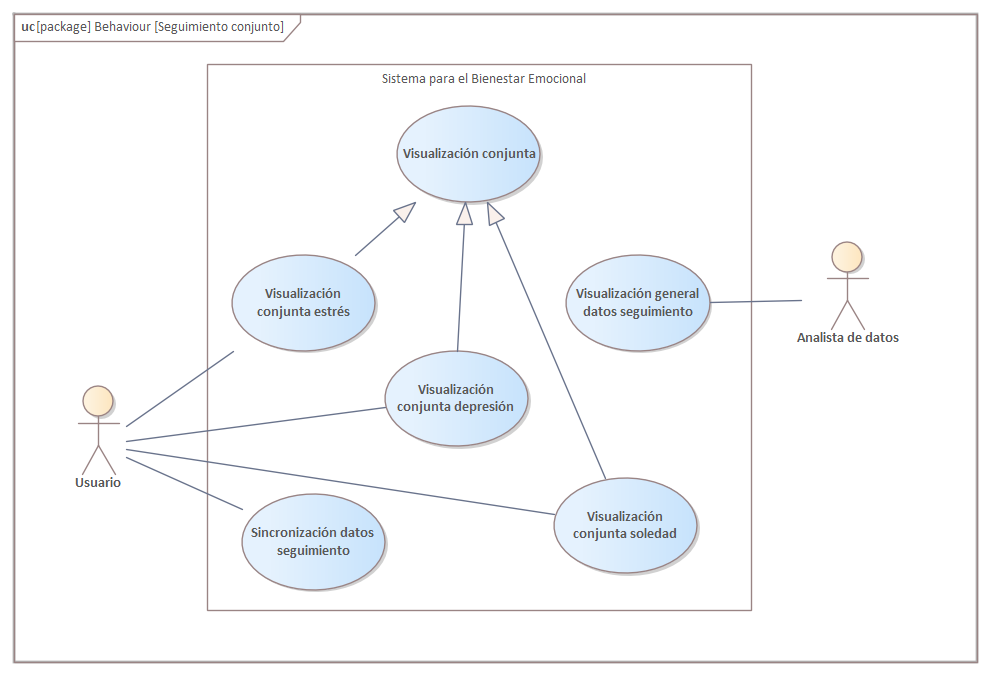
\includegraphics[width=1\textwidth]{figures/diseno/casos_uso/Seguimiento conjunto.png}
                \caption{Diagrama de casos de uso de la \textit{feature} \textbf{F-4}}
                \label{figure:diagrama_casos_uso:f4}
            \end{figure}

            Nuevamente se dispone de un diagrama que refleja cierta generalización en los casos de uso. En este caso, el caso de uso \textit{Visualización conjunta} refleja la enorme similaridad entre las diferentes visualizaciones, como se podrá vislumbrar en las especificaciones detalladas. 

            Del diagrama anterior se pueden extraer los siguientes casos de uso asociados con los diferentes actores:

            \begin{enumerate}[resume=casos-uso,label=\textbf{\texttt{CU-\arabic*}}]
                \item \label{disenio:casos_uso:sincronizacion_seguimiento} Sincronización de los datos de seguimiento
                \item \label{disenio:casos_uso:visualizacion_conjunta_estres} Visualización conjunta del estrés
                \item \label{disenio:casos_uso:visualizacion_conjunta_depresion} Visualización conjunta de la depresión
                \item \label{disenio:casos_uso:visualizacion_conjunta_soledad} Visualización conjunta de la soledad
                \item \label{disenio:casos_uso:visualizacion_general_seguimiento} Visualización general de los datos de seguimiento
            \end{enumerate}

            La especificación detallada de estos casos de uso se encuentran en la Tablas \ref{tabla:casos_uso:sincronizacion_seguimiento}, \ref{tabla:casos_uso:visualizacion_conjunta_estres}, \ref{tabla:casos_uso:visualizacion_conjunta_depresion}, \ref{tabla:casos_uso:visualizacion_conjunta_soledad} y \ref{tabla:casos_uso:visualizacion_general_seguimiento} respectivamente. Por otra parte, la Figura \ref{figure:diagrama_secuencia:visualizacion_conjunta} muestra el diagrama de secuencia de \textit{Visualización conjunta}, mientras que los diagramas de secuencia correspondientes a los casos de uso \ref{disenio:casos_uso:sincronizacion_seguimiento} y \ref{disenio:casos_uso:visualizacion_general_seguimiento} se pueden encontrar en las Figuras \ref{figure:diagrama_secuencia:sincronizacion_seguimiento} y  \ref{figure:diagrama_secuencia:visualizacion_general_seguimiento} respectivamente.

            \begin{figure}[h]
                \centering
                \includegraphics[width=1\textwidth]{figures/diseno/secuencia/Visualización conjunta.png}
                \caption{Diagrama de secuencia de \textit{Visualización conjunta}}
                \label{figure:diagrama_secuencia:visualizacion_conjunta}
            \end{figure}

            \begin{table}[h]
                \centering
                \begin{tabularx}{\textwidth}{|l|l|X|}
                    \hline
                    \textbf{ID:} CU-13 & \multicolumn{2}{|X|}{\textbf{Nombre}: Sincronización de datos de seguimiento} \\
                    \hline
                    \textbf{Evento activador} & \multicolumn{2}{|X|}{Activación por parte de Android del procedimiento de sincronización} \\
                    \hline
                    \textbf{Actor primario} & \multicolumn{2}{|X|}{Usuario} \\
                    \hline
                    \textbf{Precondición} & \multicolumn{2}{|X|}{El usuario ha completado la fase de bienvenida} \\
                    \hline
                    \multirow{8}{*}{\textbf{Flujo normal}} & \textbf{Paso} & \textbf{Acción} \\
                    \cline{2-3} & 1 & Para cada tipo de cuestionario \\
                    \cline{2-3} & 1.1 & La aplicación accede a todos los registros comprendidos entre la última sincronización registrada y el instante actual \\
                    \cline{2-3} & 2 & La aplicación envía al servidor los datos recopilados junto al identificador de usuario \\
                    \cline{2-3} & 3 & El servidor comprueba el formato de los datos enviados \\
                    \cline{2-3} & 4 & El servidor guarda en su base de datos la información recibida \\
                    \cline{2-3} & 5 & El servidor envía, para cada tipo de cuestionario, la marca de tiempo del último registro insertado en base de datos (o nulo si no se ha insertado ningún registro para ese tipo de dato) \\
                    \cline{2-3} & 6 & La aplicación guarda en su base de datos las marcas de tiempo recibidas junto a su tipo de datos \\
                    \hline
                    \textbf{Flujo alternativo} & \multicolumn{2}{|X|}{Ninguno} \\
                    \hline
                    \textbf{Postcondición} & \multicolumn{2}{|X|}{Ninguna} \\
                    \hline
                    \multirow{3}{*}{\textbf{Excepciones}}  & \textbf{Paso} & \textbf{Acción} \\
                    \cline{2-3} & 2 & Si no se puede enviar correctamente la información, el caso de uso termina \\
                    \cline{2-3} & 3 & Si el formato de los datos enviados es inválido, el servidor envía un código de error y el caso de uso termina \\
                    \hline
                    \caption{Especificación del caso de uso \ref{disenio:casos_uso:sincronizacion_seguimiento}}
                    \label{tabla:casos_uso:sincronizacion_seguimiento}
                \end{tabularx}
            \end{table}

            \begin{figure}[h]
                \centering
                \includegraphics[width=1\textwidth]{figures/diseno/secuencia/Sincronización datos seguimiento.png}
                \caption{Diagrama de secuencia de \ref{disenio:casos_uso:sincronizacion_seguimiento}}
                \label{figure:diagrama_secuencia:sincronizacion_seguimiento}
            \end{figure}

            \begin{table}[h]
                \centering
                \begin{tabularx}{\textwidth}{|l|l|X|}
                    \hline
                    \textbf{ID:} CU-14 & \multicolumn{2}{|X|}{\textbf{Nombre}: Visualización conjunta del estrés} \\
                    \hline
                    \textbf{Evento activador} & \multicolumn{2}{|X|}{El usuario accede a la ventana de visualización conjunta de estrés} \\
                    \hline
                    \textbf{Actor primario} & \multicolumn{2}{|X|}{Usuario} \\
                    \hline
                    \textbf{Precondición} & \multicolumn{2}{|X|}{El usuario ha completado la fase de bienvenida} \\
                    \hline
                    \multirow{6}{*}{\textbf{Flujo normal}} & \textbf{Paso} & \textbf{Acción} \\
                    \cline{2-3} & 1 & La aplicación obtiene del servidor la media de la puntuación de los cuestionarios de estrés del día anterior, de los últimos siete días y de cada día de la semana actual \\
                    \cline{2-3} & 2.1 & La aplicación muestra la media de la puntuación de los cuestionarios de estrés del día anterior y su nivel cualitativo \\
                    \cline{2-3} & 2.2 & La aplicación muestra la media de la puntuación de los cuestionarios de estrés de los últimos siete días y su nivel cualitativo \\
                    \cline{2-3} & 2.3 & La aplicación muestra la media de la puntuación de los cuestionarios de estrés para cada día de la semana actual \\
                    \cline{2-3} & 3 & El usuario visualiza los datos hasta que sale de la ventana, finalizando el caso de uso \\
                    \hline
                    \textbf{Flujo alternativo} & \multicolumn{2}{|X|}{Ninguno} \\
                    \hline
                    \textbf{Postcondición} & \multicolumn{2}{|X|}{Ninguna} \\
                    \hline
                    \multirow{4}{*}{\textbf{Excepciones}}  & \textbf{Paso} & \textbf{Acción} \\
                    \cline{2-3} & 2.1 & Si no hay puntuaciones de los cuestionarios de estrés del día anterior, se asumirá media y nivel nulos \\
                    \cline{2-3} & 2.2 & Si no hay puntuaciones de los cuestionarios de estrés de los últimos siete días, se asumirá media y nivel nulos \\
                    \cline{2-3} & 2.3 & Si no hay puntuaciones de los cuestionarios de estrés de la semana actual, se asumirá media nula \\
                    \hline
                    \caption{Especificación del caso de uso \ref{disenio:casos_uso:visualizacion_conjunta_estres}}
                    \label{tabla:casos_uso:visualizacion_conjunta_estres}
                \end{tabularx}
            \end{table}

            \begin{table}[h]
                \centering
                \begin{tabularx}{\textwidth}{|l|l|X|}
                    \hline
                    \textbf{ID:} CU-15 & \multicolumn{2}{|X|}{\textbf{Nombre}: Visualización conjunta de la depresión} \\
                    \hline
                    \textbf{Evento activador} & \multicolumn{2}{|X|}{El usuario accede a la ventana de visualización conjunta de depresión} \\
                    \hline
                    \textbf{Actor primario} & \multicolumn{2}{|X|}{Usuario} \\
                    \hline
                    \textbf{Precondición} & \multicolumn{2}{|X|}{El usuario ha completado la fase de bienvenida y ha permitido la monitorización de la depresión} \\
                    \hline
                    \multirow{6}{*}{\textbf{Flujo normal}} & \textbf{Paso} & \textbf{Acción} \\
                    \cline{2-3} & 1 & La aplicación obtiene del servidor la media de la puntuación de los cuestionarios de depresión del día anterior, de los últimos siete días y de cada día de la semana actual \\
                    \cline{2-3} & 2.1 & La aplicación muestra la media de la puntuación de los cuestionarios de depresión del día anterior y su nivel cualitativo \\
                    \cline{2-3} & 2.2 & La aplicación muestra la media de la puntuación de los cuestionarios de depresión de los últimos siete días y su nivel cualitativo \\
                    \cline{2-3} & 2.3 & La aplicación muestra la media de la puntuación de los cuestionarios de depresión para cada día de la semana actual \\
                    \cline{2-3} & 3 & El usuario visualiza los datos hasta que sale de la ventana, finalizando el caso de uso \\
                    \hline
                    \textbf{Flujo alternativo} & \multicolumn{2}{|X|}{Ninguno} \\
                    \hline
                    \textbf{Postcondición} & \multicolumn{2}{|X|}{Ninguna} \\
                    \hline
                    \multirow{4}{*}{\textbf{Excepciones}}  & \textbf{Paso} & \textbf{Acción} \\
                    \cline{2-3} & 2.1 & Si no hay puntuaciones de los cuestionarios de depresión del día anterior, se asumirá media y nivel nulos \\
                    \cline{2-3} & 2.2 & Si no hay puntuaciones de los cuestionarios de depresión de los últimos siete días, se asumirá media y nivel nulos \\
                    \cline{2-3} & 2.3 & Si no hay puntuaciones de los cuestionarios de depresión de la semana actual, se asumirá media nula \\
                    \hline
                    \caption{Especificación del caso de uso \ref{disenio:casos_uso:visualizacion_conjunta_depresion}}
                    \label{tabla:casos_uso:visualizacion_conjunta_depresion}
                \end{tabularx}
            \end{table}

            \begin{table}[h]
                \centering
                \begin{tabularx}{\textwidth}{|l|l|X|}
                    \hline
                    \textbf{ID:} CU-16 & \multicolumn{2}{|X|}{\textbf{Nombre}: Visualización conjunta de la soledad} \\
                    \hline
                    \textbf{Evento activador} & \multicolumn{2}{|X|}{El usuario accede a la ventana de visualización conjunta de soledad} \\
                    \hline
                    \textbf{Actor primario} & \multicolumn{2}{|X|}{Usuario} \\
                    \hline
                    \textbf{Precondición} & \multicolumn{2}{|X|}{El usuario ha completado la fase de bienvenida y ha permitido la monitorización de la soledad} \\
                    \hline
                    \multirow{6}{*}{\textbf{Flujo normal}} & \textbf{Paso} & \textbf{Acción} \\
                    \cline{2-3} & 1 & La aplicación obtiene del servidor la media de la puntuación de los cuestionarios de soledad del día anterior, de los últimos siete días y de cada día de la semana actual \\
                    \cline{2-3} & 2.1 & La aplicación muestra la media de la puntuación de los cuestionarios de soledad del día anterior y su nivel cualitativo \\
                    \cline{2-3} & 2.2 & La aplicación muestra la media de la puntuación de los cuestionarios de soledad de los últimos siete días y su nivel cualitativo \\
                    \cline{2-3} & 2.3 & La aplicación muestra la media de la puntuación de los cuestionarios de soledad para cada día de la semana actual \\
                    \cline{2-3} & 3 & El usuario visualiza los datos hasta que sale de la ventana, finalizando el caso de uso \\
                    \hline
                    \textbf{Flujo alternativo} & \multicolumn{2}{|X|}{Ninguno} \\
                    \hline
                    \textbf{Postcondición} & \multicolumn{2}{|X|}{Ninguna} \\
                    \hline
                    \multirow{4}{*}{\textbf{Excepciones}}  & \textbf{Paso} & \textbf{Acción} \\
                    \cline{2-3} & 2.1 & Si no hay puntuaciones de los cuestionarios de soledad del día anterior, se asumirá media y nivel nulos \\
                    \cline{2-3} & 2.2 & Si no hay puntuaciones de los cuestionarios de soledad de los últimos siete días, se asumirá media y nivel nulos \\
                    \cline{2-3} & 2.3 & Si no hay puntuaciones de los cuestionarios de soledad de la semana actual, se asumirá media nula \\
                    \hline
                    \caption{Especificación del caso de uso \ref{disenio:casos_uso:visualizacion_conjunta_soledad}}
                    \label{tabla:casos_uso:visualizacion_conjunta_soledad}
                \end{tabularx}
            \end{table}

            \begin{table}[h]
                \centering
                \begin{tabularx}{\textwidth}{|l|l|X|}
                    \hline
                    \textbf{ID:} CU-17 & \multicolumn{2}{|X|}{\textbf{Nombre}: Visualización general de los datos de seguimiento} \\
                    \hline
                    \textbf{Evento activador} & \multicolumn{2}{|X|}{El analista de datos ha indicado visualizar los datos generales de seguimiento} \\
                    \hline
                    \textbf{Actor primario} & \multicolumn{2}{|X|}{Analista de datos} \\
                    \hline
                    \textbf{Precondición} & \multicolumn{2}{|X|}{Ninguna} \\
                    \hline
                    \multirow{3}{*}{\textbf{Flujo normal}} & \textbf{Paso} & \textbf{Acción} \\
                    \cline{2-3} & 1 & El analista de datos se conecta a la base de datos del servidor \\
                    \cline{2-3} & 2 & El analista de datos puede consultar para cada identificador de usuario, los datos de los cuestionarios realizados \\
                    \hline
                    \textbf{Flujo alternativo} & \multicolumn{2}{|X|}{Ninguno} \\
                    \hline
                    \textbf{Postcondición} & \multicolumn{2}{|X|}{Ninguna} \\
                    \hline
                    Exepciones & \multicolumn{2}{|X|}{Ninguna} \\
                    \hline
                    \caption{Especificación del caso de uso \ref{disenio:casos_uso:visualizacion_general_seguimiento}}
                    \label{tabla:casos_uso:visualizacion_general_seguimiento}
                \end{tabularx}
            \end{table}
            
            \begin{figure}[h]
                \centering
                \includegraphics[width=0.75\textwidth]{figures/diseno/secuencia/Visualización general seguimiento.png}
                \caption{Diagrama de secuencia de \ref{disenio:casos_uso:visualizacion_general_seguimiento}}
                \label{figure:diagrama_secuencia:visualizacion_general_seguimiento}
            \end{figure}

            \clearpage  % Asegura que todas las figuras y tablas pendientes se impriman antes de continuar.
            
        \subsection*{Feature 5: Recopilación del histórico}
            Por último esta característica es exclusiva al usuario y describe la funcionalidad relativa a la visualización de estadísticas detalladas sobre las diferentes enfermedades. El diagrama de casos de uso de esta \textit{feature} se puede encontrar en la Figura \ref{figure:diagrama_casos_uso:f5}.

            \begin{figure}[h]
                \centering
                \includegraphics[width=1\textwidth]{figures/diseno/casos_uso/Recopilación historico.png}
                \caption{Diagrama de casos de uso de la \textit{feature} \textbf{F-5}}
                \label{figure:diagrama_casos_uso:f5}
            \end{figure}

             Del diagrama anterior se pueden extraer los siguientes casos de uso:

            \begin{enumerate}[resume=casos-uso,label=\textbf{\texttt{CU-\arabic*}}]
                \item \label{disenio:casos_uso:visualizacion_estadistica_estres} Visualización estadística de los datos de estrés
                \item \label{disenio:casos_uso:visualizacion_estadistica_depresion} Visualización estadística de los datos de depresión
                \item \label{disenio:casos_uso:visualizacion_estadistica_soledad} Visualización estadística de los datos de soledad
            \end{enumerate}

            Los tres casos de uso con los que el usuario está asociado son generalizados por \textit{Visualización estadística}, el cual será modelado como un diagrama de secuencia en la Figura \ref{figure:diagrama_secuencia:visualizacion_estadistica}, mientras que la especificación detallada de los casos de uso asociados con el usuario se encuentran en la Tablas \ref{tabla:casos_uso:visualizacion_estadistica_estres}, \ref{tabla:casos_uso:visualizacion_estadistica_depresion} y \ref{tabla:casos_uso:visualizacion_estadistica_soledad} respectivamente.

            \begin{figure}[h]
                \centering
                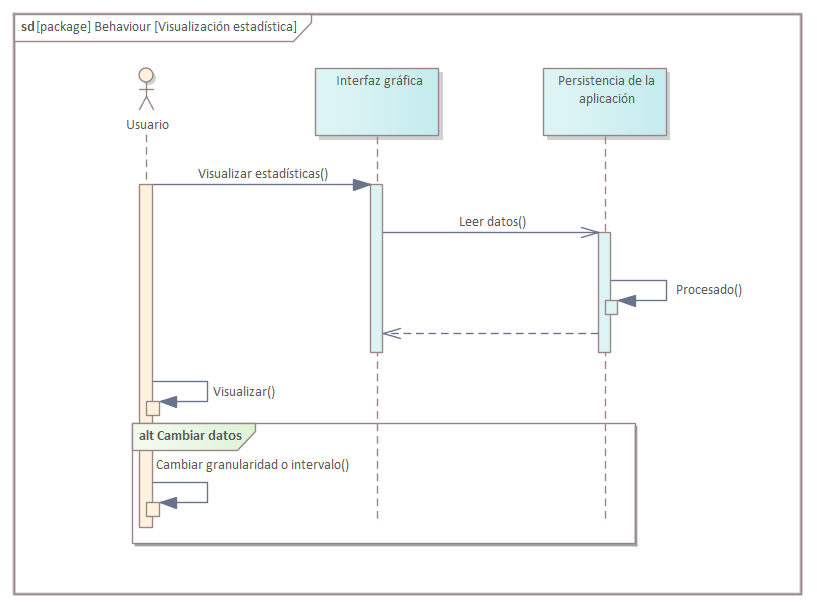
\includegraphics[width=1\textwidth]{figures/diseno/secuencia/Visualización estadística.png}
                \caption{Diagrama de secuencia de \textit{Visualización estadística}}
                \label{figure:diagrama_secuencia:visualizacion_estadistica}
            \end{figure}
            
            \begin{table}[h]
                \centering
                \begin{tabularx}{\textwidth}{|l|l|X|}
                    \hline
                    \textbf{ID:} CU-18 & \multicolumn{2}{|X|}{\textbf{Nombre}: Visualización estadística de los datos de estrés} \\
                    \hline
                    \textbf{Evento activador} & \multicolumn{2}{|X|}{El usuario accede a la ventana de histórico de la aplicación} \\
                    \hline
                    \textbf{Actor primario} & \multicolumn{2}{|X|}{Usuario} \\
                    \hline
                    \textbf{Precondición} & \multicolumn{2}{|X|}{El usuario ha completado la fase de bienvenida} \\
                    \hline
                    \multirow{7}{*}{\textbf{Flujo normal}} & \textbf{Paso} & \textbf{Acción} \\
                    \cline{2-3} & 1 & La aplicación asume por defecto que los datos se agruparán por día y el intervalo de fechas son los últimos siete días \\
                    \cline{2-3} & 2 & La aplicación acede a los datos de los cuestionarios de estrés del intervalo de fechas \\
                    \cline{2-3} & 3 & La aplicación procesa los datos leídos, agrupando los datos según la granularidad y realizando la media \\
                    \cline{2-3} & 4 & La aplicación presenta los datos procesados \\
                    \cline{2-3} & 5 & El usuario visualiza los datos \\
                    \cline{2-3} & 6 & El usuario finaliza la visualización de los datos \\
                    \hline
                    \multirow{5}{*}{\textbf{Flujo alternativo}} & \textbf{Paso} & \textbf{Acción} \\
                    \cline{2-3} & 3 & Si en alguna de las agrupaciones no hay datos con lo que realizar la media, se realiza la siguiente imputación \\
                    \cline{2-3} & 3.1 & Si hay datos en las tres agrupaciones previas, se realiza la media de la puntuación de estas \\
                    \cline{2-3} & 3.2 & Si no hay datos en las tres agrupaciones previas, se realiza la media de la puntuación de todas las agrupaciones que tengan datos \\
                    \cline{2-3} & 6 & El usuario puede cambiar la granularidad de los datos, volviendo al paso 3 del flujo normal; o el intervalo de fechas, volviendo al paso 2 del flujo normal \\
                    \hline
                    \textbf{Postcondición} & \multicolumn{2}{|X|}{Ninguna} \\
                    \hline
                    Exepciones & \multicolumn{2}{|X|}{Ninguna} \\
                    \hline
                    \caption{Especificación del caso de uso \ref{disenio:casos_uso:visualizacion_estadistica_estres}}
                    \label{tabla:casos_uso:visualizacion_estadistica_estres}
                \end{tabularx}
            \end{table}

            \begin{table}[h]
                \centering
                \begin{tabularx}{\textwidth}{|l|l|X|}
                    \hline
                    \textbf{ID:} CU-19 & \multicolumn{2}{|X|}{\textbf{Nombre}: Visualización estadística de los datos de depresión} \\
                    \hline
                    \textbf{Evento activador} & \multicolumn{2}{|X|}{El usuario accede a la ventana de histórico de la aplicación} \\
                    \hline
                    \textbf{Actor primario} & \multicolumn{2}{|X|}{Usuario} \\
                    \hline
                    \textbf{Precondición} & \multicolumn{2}{|X|}{El usuario ha completado la fase de bienvenida y ha permitido la monitorización de la depresión} \\
                    \hline
                    \multirow{7}{*}{\textbf{Flujo normal}} & \textbf{Paso} & \textbf{Acción} \\
                    \cline{2-3} & 1 & La aplicación asume por defecto que los datos se agruparán por día y el intervalo de fechas son los últimos siete días \\
                    \cline{2-3} & 2 & La aplicación acede a los datos de los cuestionarios de depresión del intervalo de fechas \\
                    \cline{2-3} & 3 & La aplicación procesa los datos leídos, agrupando los datos según la granularidad y realizando la media \\
                    \cline{2-3} & 4 & La aplicación presenta los datos procesados \\
                    \cline{2-3} & 5 & El usuario visualiza los datos \\
                    \cline{2-3} & 6 & El usuario finaliza la visualización de los datos \\
                    \hline
                    \multirow{5}{*}{\textbf{Flujo alternativo}} & \textbf{Paso} & \textbf{Acción} \\
                    \cline{2-3} & 3 & Si en alguna de las agrupaciones no hay datos con lo que realizar la media, se realiza la siguiente imputación \\
                    \cline{2-3} & 3.1 & Si hay datos en las tres agrupaciones previas, se realiza la media de la puntuación de estas \\
                    \cline{2-3} & 3.2 & Si no hay datos en las tres agrupaciones previas, se realiza la media de la puntuación de todas las agrupaciones que tengan datos \\
                    \cline{2-3} & 6 & El usuario puede cambiar la granularidad de los datos, volviendo al paso 3 del flujo normal; o el intervalo de fechas, volviendo al paso 2 del flujo normal \\
                    \hline
                    \textbf{Postcondición} & \multicolumn{2}{|X|}{Ninguna} \\
                    \hline
                    Exepciones & \multicolumn{2}{|X|}{Ninguna} \\
                    \hline
                    \caption{Especificación del caso de uso \ref{disenio:casos_uso:visualizacion_estadistica_depresion}}
                    \label{tabla:casos_uso:visualizacion_estadistica_depresion}
                \end{tabularx}
            \end{table}
            
            \begin{table}[h]
                \centering
                \begin{tabularx}{\textwidth}{|l|l|X|}
                    \hline
                    \textbf{ID:} CU-20 & \multicolumn{2}{|X|}{\textbf{Nombre}: Visualización estadística de los datos de soledad} \\
                    \hline
                    \textbf{Evento activador} & \multicolumn{2}{|X|}{El usuario accede a la ventana de histórico de la aplicación} \\
                    \hline
                    \textbf{Actor primario} & \multicolumn{2}{|X|}{Usuario} \\
                    \hline
                    \textbf{Precondición} & \multicolumn{2}{|X|}{El usuario ha completado la fase de bienvenida y ha permitido la monitorización de la soledad} \\
                    \hline
                    \multirow{7}{*}{\textbf{Flujo normal}} & \textbf{Paso} & \textbf{Acción} \\
                    \cline{2-3} & 1 & La aplicación asume por defecto que los datos se agruparán por día y el intervalo de fechas son los últimos siete días \\
                    \cline{2-3} & 2 & La aplicación acede a los datos de los cuestionarios de soledad del intervalo de fechas \\
                    \cline{2-3} & 3 & La aplicación procesa los datos leídos, agrupando los datos según la granularidad y realizando la media \\
                    \cline{2-3} & 4 & La aplicación presenta los datos procesados \\
                    \cline{2-3} & 5 & El usuario visualiza los datos \\
                    \cline{2-3} & 6 & El usuario finaliza la visualización de los datos \\
                    \hline
                    \multirow{5}{*}{\textbf{Flujo alternativo}} & \textbf{Paso} & \textbf{Acción} \\
                    \cline{2-3} & 3 & Si en alguna de las agrupaciones no hay datos con lo que realizar la media, se realiza la siguiente imputación \\
                    \cline{2-3} & 3.1 & Si hay datos en las tres agrupaciones previas, se realiza la media de la puntuación de estas \\
                    \cline{2-3} & 3.2 & Si no hay datos en las tres agrupaciones previas, se realiza la media de la puntuación de todas las agrupaciones que tengan datos \\
                    \cline{2-3} & 6 & El usuario puede cambiar la granularidad de los datos, volviendo al paso 3 del flujo normal; o el intervalo de fechas, volviendo al paso 2 del flujo normal \\
                    \hline
                    \textbf{Postcondición} & \multicolumn{2}{|X|}{Ninguna} \\
                    \hline
                    Exepciones & \multicolumn{2}{|X|}{Ninguna} \\
                    \hline
                    \caption{Especificación del caso de uso \ref{disenio:casos_uso:visualizacion_estadistica_soledad}}
                    \label{tabla:casos_uso:visualizacion_estadistica_soledad}
                \end{tabularx}
            \end{table}
            
            \clearpage  % Asegura que todas las figuras y tablas pendientes se impriman antes de continuar.
            
    
    \section{Diseño del sistema}
    
        \subsection{Componentes del sistema}

            El sistema contará con tres componentes principales, ya planteados en la sección \ref{req:descripcion:perspectiva}: una aplicación móvil, un componente servidor y un dispositivo \gls{wearable}, siendo este último de carácter opcional para el usuario. En la Figura \ref{figure:diseno:componentes} se puede encontrar una representación gráfica de los mismos y de sus interacciones básicas.
            
            \begin{figure}[h]
                \centering
                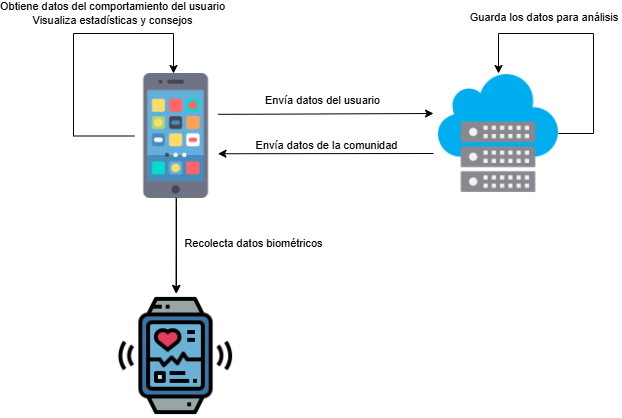
\includegraphics[width=0.75\textwidth]{figures/diseno/Componentes.png}
                \caption{Visión general de los componentes del sistema}
                \label{figure:diseno:componentes}
            \end{figure}
            
            En primer lugar, la aplicación móvil es el núcleo principal del proyecto y centralizará todas las interacciones con el usuario. En particular, las responsabilidades de este componente son:
            
            \begin{enumerate}
                \item Lectura de los datos extraídos por el dispositivo \gls{wearable} a través del \gls{framework} \textit{Salud Conectada}.
                \item Despliegue, realización, guardado y administración de los cuestionarios relativos a cada desorden mental. Para ello realizará el envío de notificaciones al usuario, presentará los cuestionarios, guardará el progreso de los mismos e informará al usuario si dispone de cuestionarios incompletos.
                \item Presentación del estado actual del usuario de cada enfermedad, junto a los consejos correspondientes para la mejora del mismo.
                \item Visualización de estadísticas detalladas relativas a cada desorden, tanto las correspondientes al usuario como las de la comunidad en su conjunto.
                \item Envío de los datos recogidos del usuario al servidor para su posterior análisis.
                \item Comunicación con el servidor para la obtención de los datos de la comunidad.
                \item Gestión de aspectos transversales relacionados con el usuario, tales como la presentación del tutorial de bienvenida, la administración de los ajustes del usuario  o la visualización de la información legal.
            \end{enumerate}
                
            Por otra parte, el componente servidor contendrá todas las interacciones del analista de datos. Fundamentalmente se encargará tanto de recibir y guardar los datos de los usuarios como de suministrar los datos relativos a la comunidad a los usuarios, estando localizado este componente en un servidor de la \gls{etsisi}.
            
            Por último, el dispositivo \gls{wearable} es el encargado de la extracción de datos biométricos del usuario. Al ser escogido el uso de \textit{Salud Conectada}, el sistema no se encargará de la extracción de estos datos, reutilizando la implementación del fabricante del dispositivo. Por tanto, se puede considerar a este componente como una \textit{caja negra}, realizando lecturas de los datos recogidos\footnote{A partir de este momento se considerará que el sistema consta de dos componentes principales (aplicación y servidor) a nivel práctico, ya que al ser accedidos los datos mediante \textit{Salud Conectada} no es necesario desarrollar en la práctica un tercer componente independiente.}.

        \subsection{Arquitectura}

            La arquitectura de este proyecto se ha diseñado utilizando los modelos cliente-servidor y multicapa. El primero de ellos permite plantear las interacciones entre la aplicación y el servidor, realizándose en este caso mediante una \gls{api}; mientras que el diseño basado en capas permite organizar los diferentes módulos software dentro de cada componente. 

            En primer lugar, las capas que se han planteado para el componente aplicación son:

            \begin{itemize}
                \item Capa \textit{presentación}: se encarga de la interacción con el usuario en sus diversas formas. Aquí se pueden encontrar elementos como las pantallas de la aplicación, las notificaciones y las estadísticas. 
                \item Capa \textit{dominio}: implementa funciones relacionadas con el proceso de datos, la comunicación con el servidor o la simplificación del acceso a datos mediante la creación de repositorios.
                \item Capa \textit{datos}: en esta última capa se pueden localizar las funciones de lectura de datos de diversas fuentes, tales como de los \glspl{wearable} o de base de datos, o la implementación de los modelos de los cuestionarios detallados en los Anexos \ref{chapter:cuestionarios_diarios} y \ref{chapter:cuestionarios_puntuales}. 
            \end{itemize}

            La representación gráfica de la arquitectura de capas del componente aplicación se puede encontrar en la Figura \ref{figure:disenio:arquitectura_app}.
        
            \begin{figure}[h]
                \centering
                \includegraphics[width=0.66\textwidth]{figures/diseno/Aplicación pila.png}
                \caption{Arquitectura básica de la aplicación}
                \label{figure:disenio:arquitectura_app}
            \end{figure}
            
            Por otra parte, la arquitectura básica del componente servidor también consta de tres capas, a saber: 
            \begin{itemize}
                \item Capa \gls{api}: contiene los \textit{endpoints} que se exponen al exterior, es decir, la interfaz externa.
                \item Capa de dominio, en la cual se puede encontrar los módulos \textit{validator} y \textit{response}, los cuales se encargan de verificar las peticiones recibidas y de la generación de las respuestas respectivamente.
                \item Capa de persistencia, donde se implementan los accesos a las diferentes colecciones de datos.
            \end{itemize}

            Análogamente, se puede encontrar la representación gráfica de las capas del componente servidor en la Figura \ref{figure:disenio:arquitectura_servidor}.
            
            \begin{figure}[h]
                \centering
                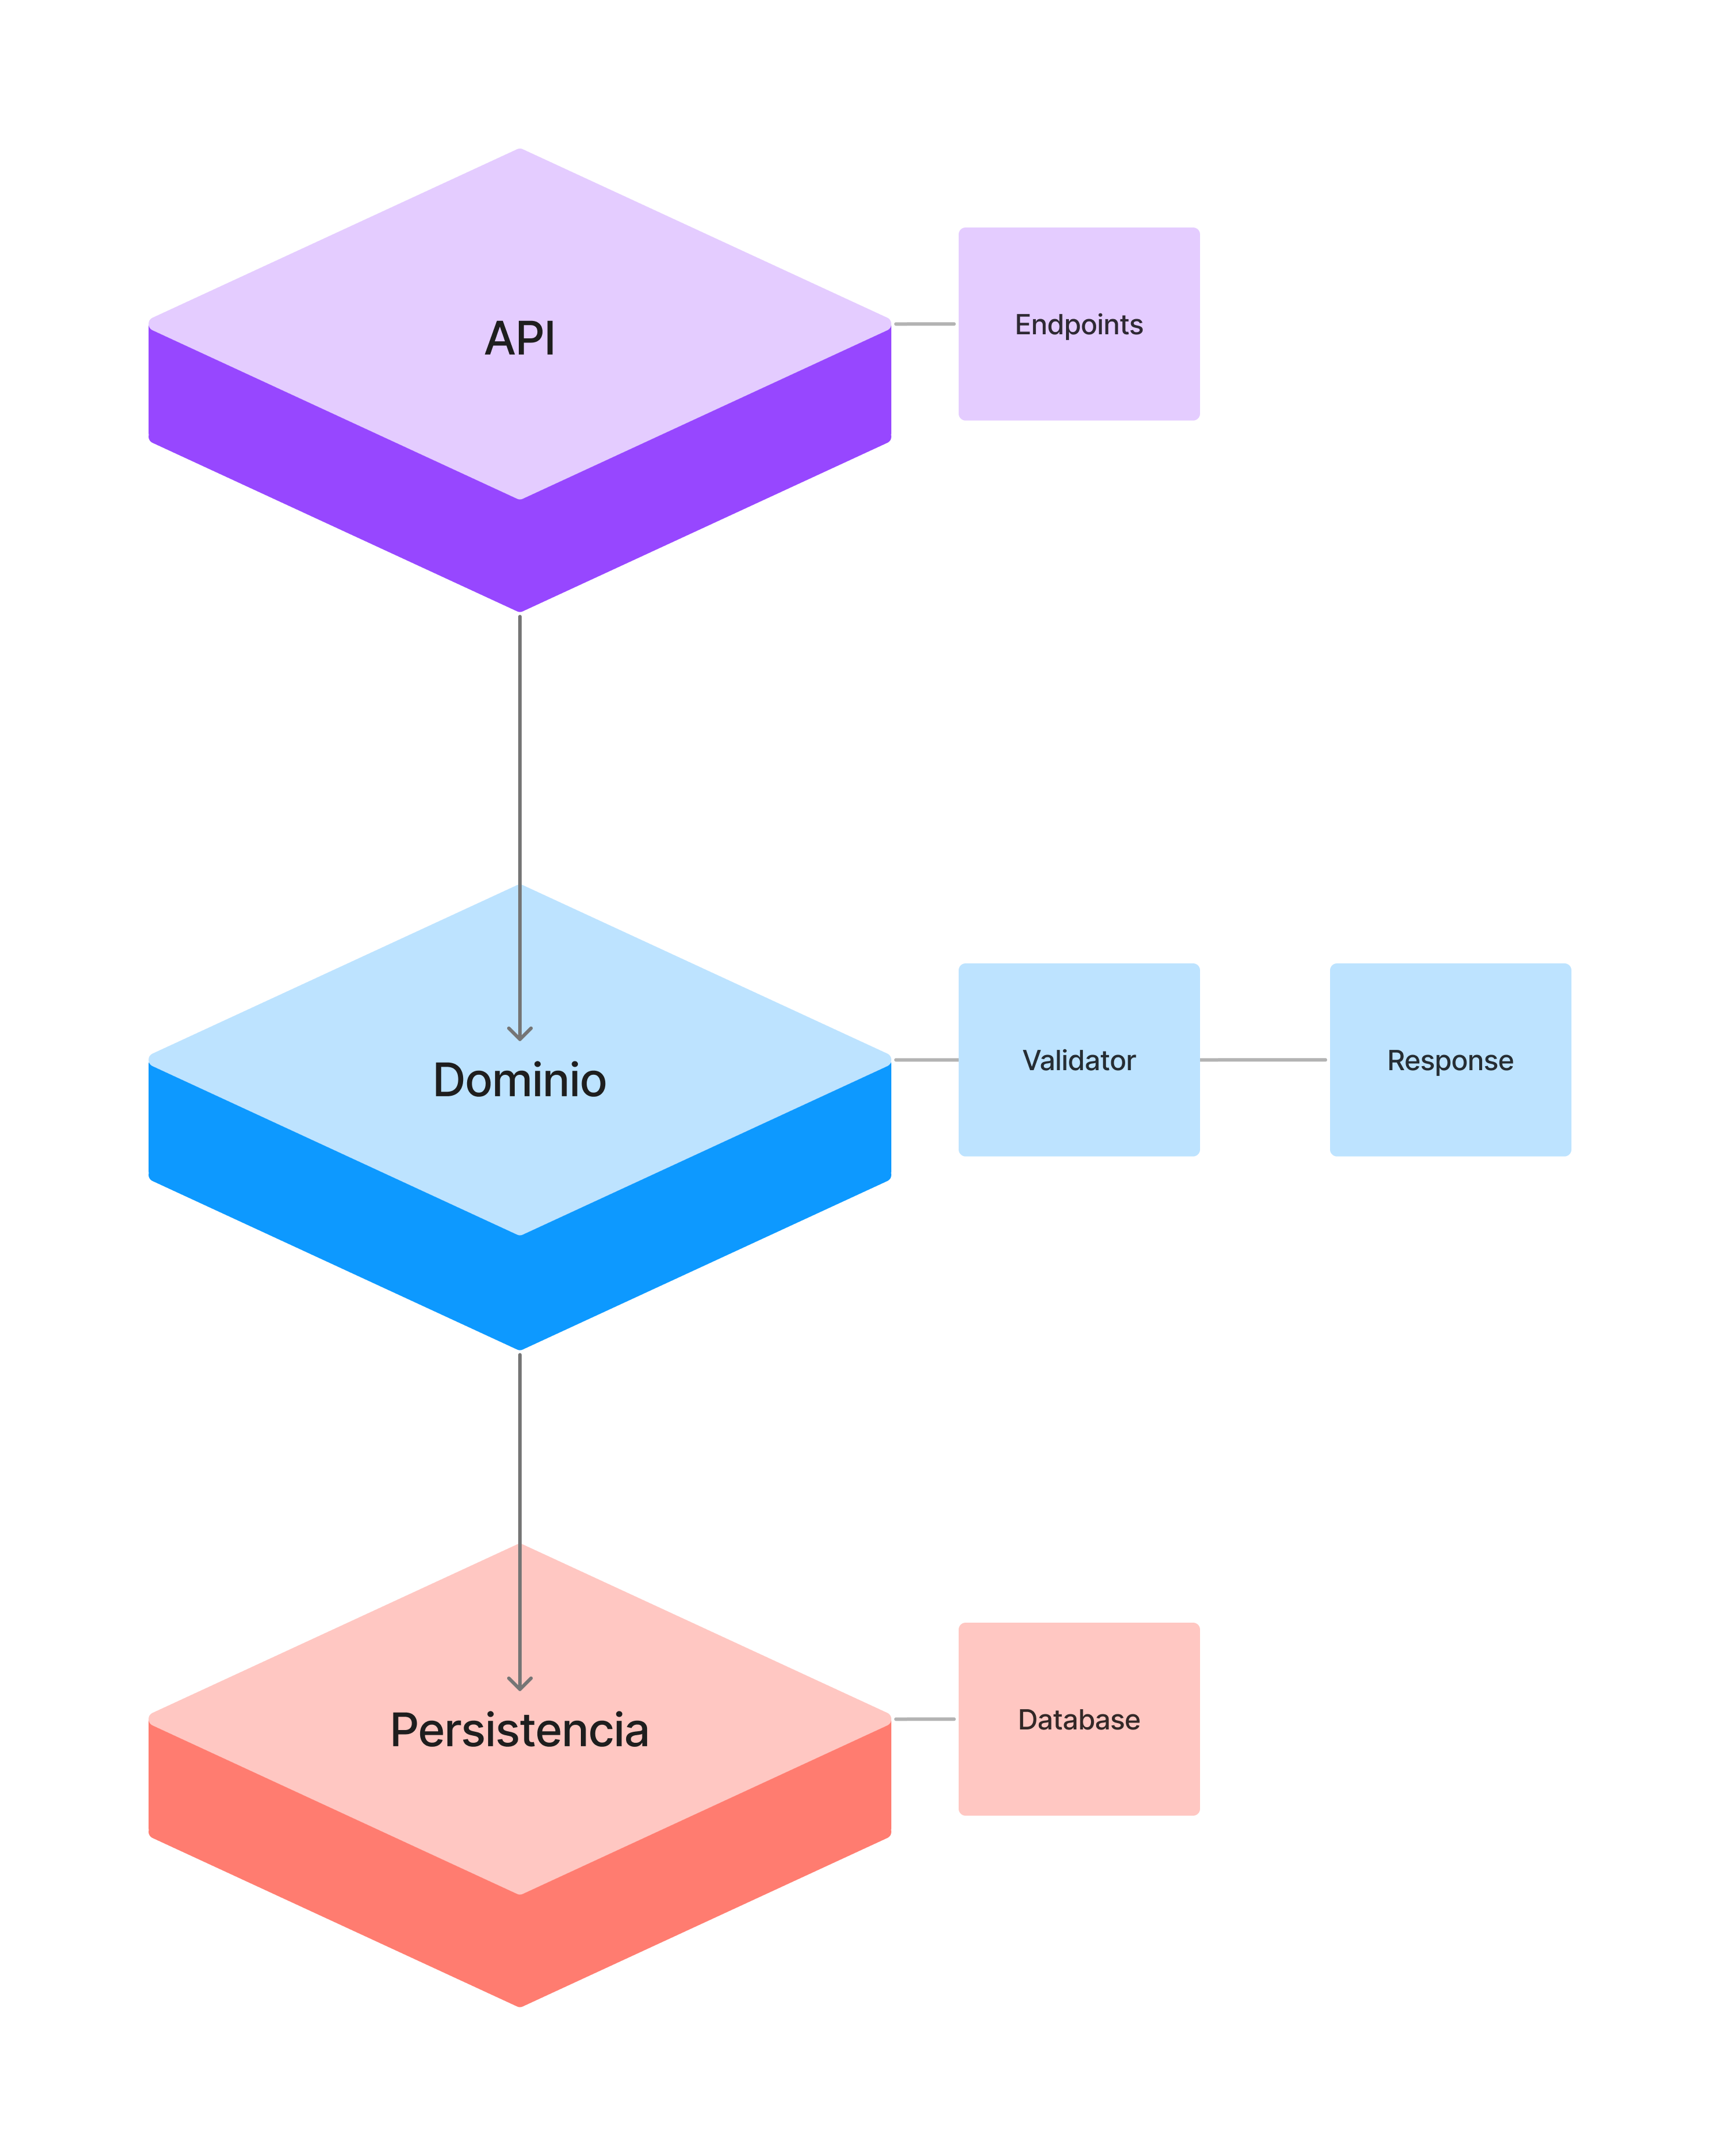
\includegraphics[width=0.66\textwidth]{figures/diseno/Servidor pila.png}
                \caption{Arquitectura básica del servidor}
                \label{figure:disenio:arquitectura_servidor}
            \end{figure}
            
    
        \subsection{Persistencia}

            Continuando con el diseño de la persistencia, en esta sección se presentarán los modelados tanto del componente aplicación como del servidor. En primer lugar, la persistencia del componente aplicación fue modelada mediante un diagrama entidad-relación, el cual se presenta en la Figura \ref{figure:disenio:diagrama_er}.
            
            \begin{sidewaysfigure}[h]
                \centering
                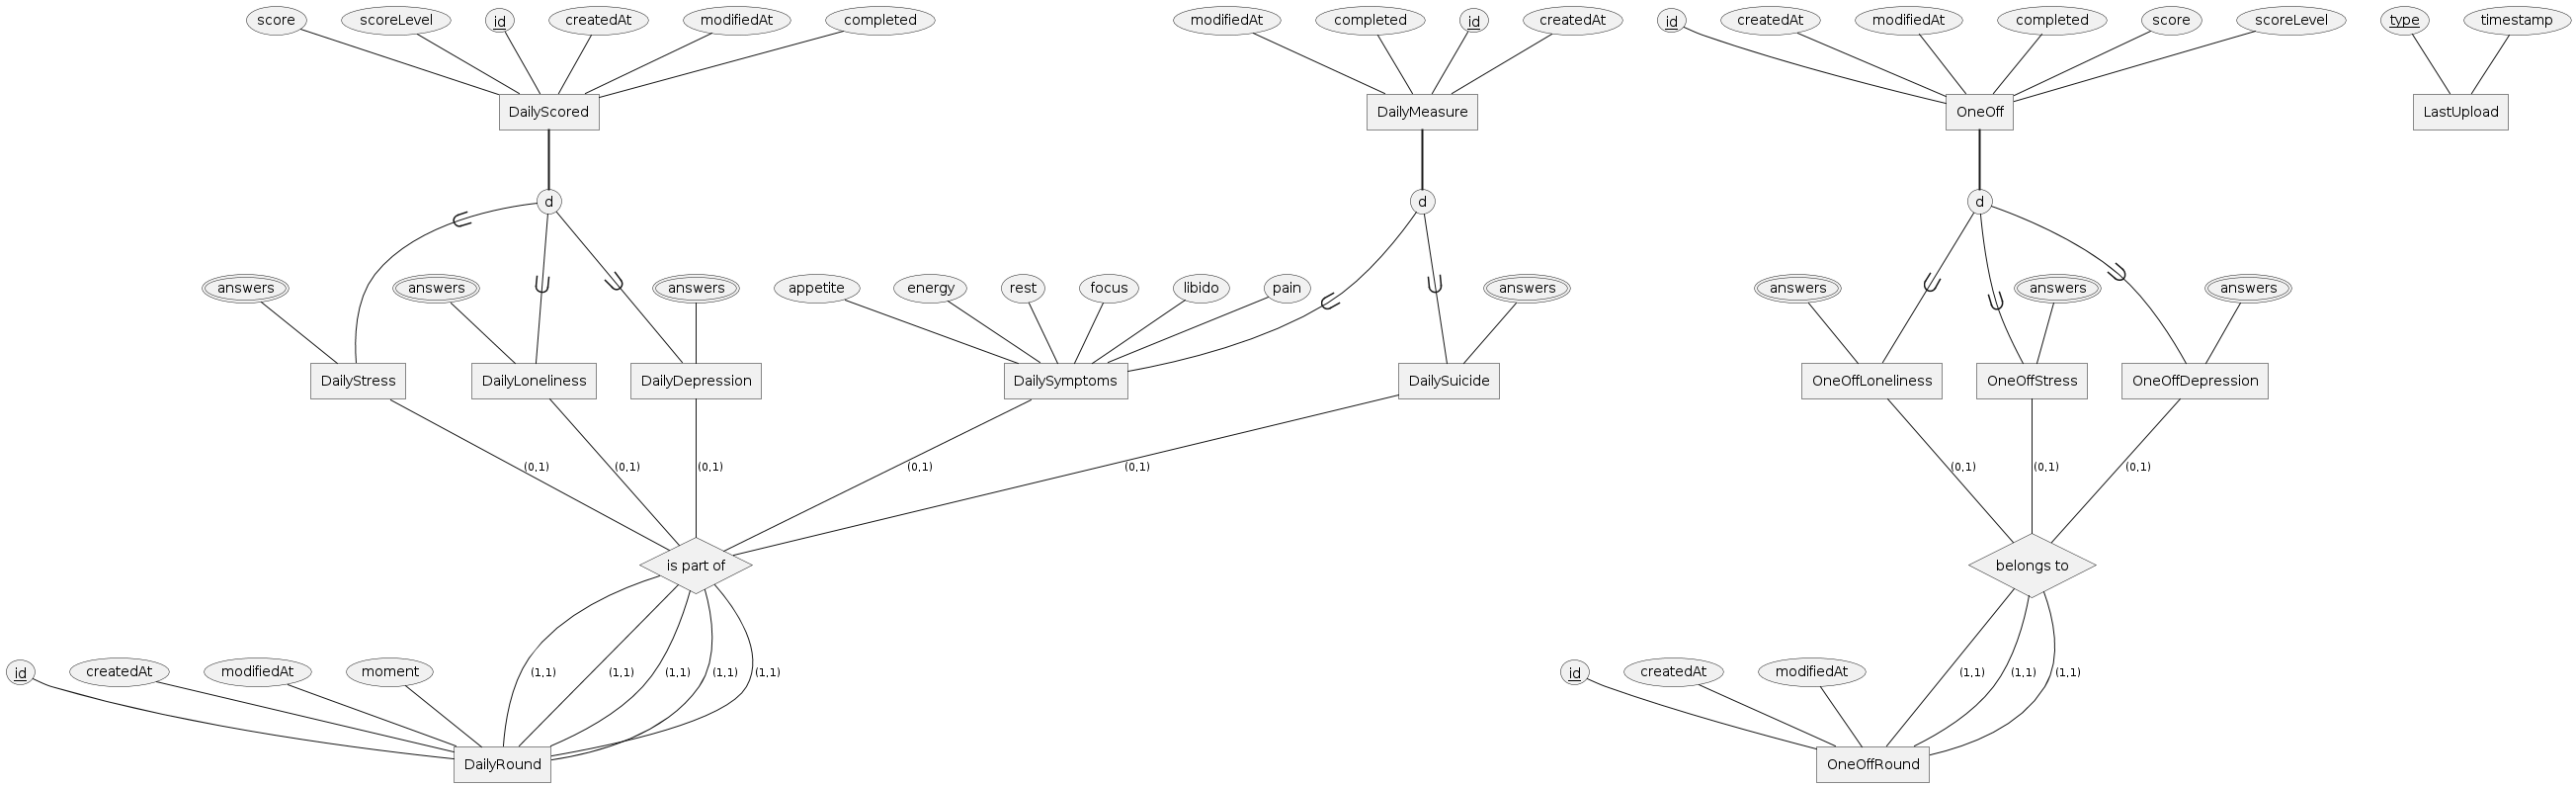
\includegraphics[width=1\textwidth]{figures/bd/ER simple.png}
                \caption{Diagrama Entidad Relación de la base de datos de la aplicación}
                \label{figure:disenio:diagrama_er}
            \end{sidewaysfigure}

            \clearpage  % Asegura que todas las figuras y tablas pendientes se impriman antes de continuar.


            Tras analizarse los diferentes diagramas de diseño, se tomó la decisión de agrupar los cuestionarios bajo el concepto de \textit{Ronda de cuestionarios}, con la finalidad clara de simplificar la implementación de los diferentes cuestionarios. Se establecieron dos tipos de rondas, a saber, diarias\footnote{Se pudo generalizar en base a los cuestionarios diarios ya que únicamente cambian los textos de los cuestionarios, por lo que se puede diferenciar entre matutino y vespertino en base de datos mediante un único atributo} y puntuales.

            Para el modelado de esta decisión de diseño, en el modelo entidad-relación fueron creadas una serie de entidades abstractas, \textit{DailyScored}, \textit{DailyMeasure} y \textit{OneOff}, las cuales representan a los cuestionarios diarios con puntuación, los cuestionarios diarios que carecen de puntuación y los cuestionarios puntuales respectivamente. Estas entidades abstractas son extendidas por los diferentes cuestionarios, siendo estas entidades derivadas agrupadas según su frecuencia en las diferentes \textit{rondas de cuestionarios}. 

            En cuanto a la persistencia de los datos en el componente servidor, al disponerse de un \gls{sgbd} no relacional fueron diseñadas tres colecciones, a saber: datos de actividad física del usuario o \textit{user data}, cuestionarios diarios o \textit{daily questionnaires} y cuestionarios puntuales o \textit{one off questionnaires}. Las Figuras \ref{figure:disenio:diagrama_user_data},  \ref{figure:disenio:diagrama_daily} y \ref{figure:disenio:diagrama_one_off} respectivamente representan el modelado de estas colecciones.

            En el caso de la colección \textit{user data}, se guarda para cada usuario los diferentes tipos de datos que se pueden recoger del \gls{wearable} en un primer nivel. En un segundo nivel se detallan los intervalos de tiempo y las medidas, estableciéndose un tercer nivel de profundidad para aquellas medidas más complejas, como las fases del sueño o las muestras de la \gls{vfc}.

            \begin{figure}[h]
                \centering
                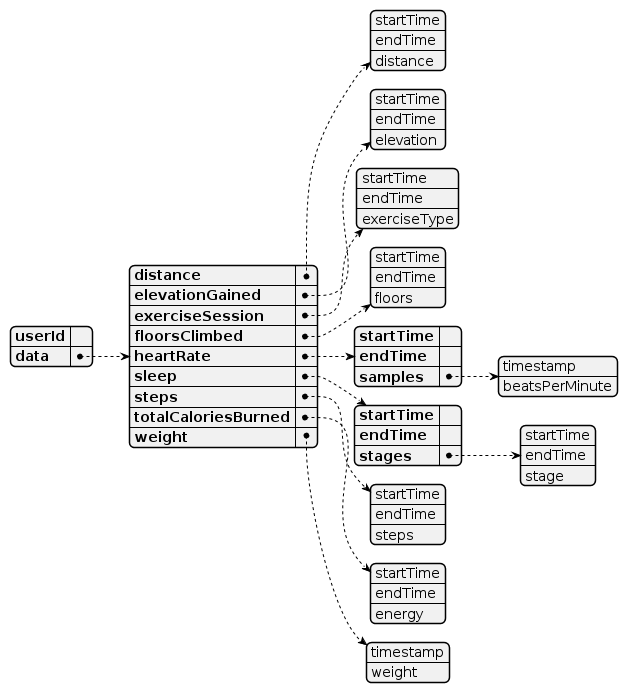
\includegraphics[width=0.75\textwidth]{figures/bd/Servidor user data.png}
                \caption{Modelado de la colección \textit{user data}}
                \label{figure:disenio:diagrama_user_data}
            \end{figure}

            En cuanto a las colecciones de los cuestionarios, se establece en el nivel raíz el identificador de usuario. Los niveles de profundidad sucesivos definen los tipos de cuestionarios y la información de cada instancia de los mismos.
    
            \begin{figure}[h]
                \centering
                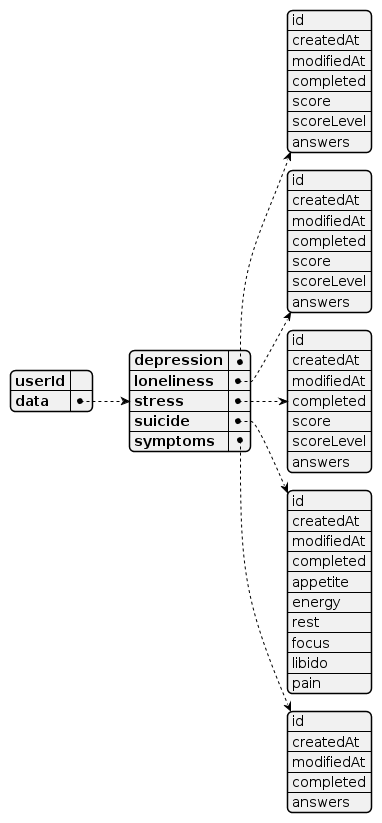
\includegraphics[width=0.5\textwidth]{figures/bd/Servidor daily questionnaires.png}
                \caption{Modelado de la colección \textit{daily questionnaires}}
                \label{figure:disenio:diagrama_daily}
            \end{figure}
            
            \begin{figure}[h]
                \centering
                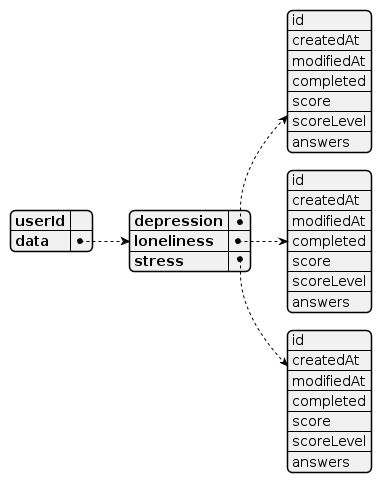
\includegraphics[width=0.5\textwidth]{figures/bd/Servidor one off questionnaires.png}
                \caption{Modelado de la colección \textit{one off questionnaires}}
                \label{figure:disenio:diagrama_one_off}
            \end{figure}
            
            Por último, para simplificar notablemente la implementación, el formato \gls{json} de estas colecciones será reutilizado para el envío de datos entre la aplicación y el servidor. 

            \clearpage  % Asegura que todas las figuras y tablas pendientes se impriman antes de continuar.
            
        \subsection{Interfaz gráfica}

            Los esquemas de colores de la interfaz gráfica de la aplicación fueron diseñados con la herramienta \textit{Material Design Builder} \cite{material_design_material_nodate-1}. Esta plataforma necesita una serie de colores principales o semilla, los cuales son utilizados en gran medida a lo largo de la aplicación.

            La selección de los colores semilla fue realizada en colaboración con la asociación de la \gls{etsisi} \textit{LevelUp}, para obtener una mayor retroalimentación e ideas para los mismos. Los colores elegidos se pueden visualizar en la Figura \ref{figure:disenio:colores_semilla}, siendo su caracterización:

            \begin{figure}[h]
                \centering
                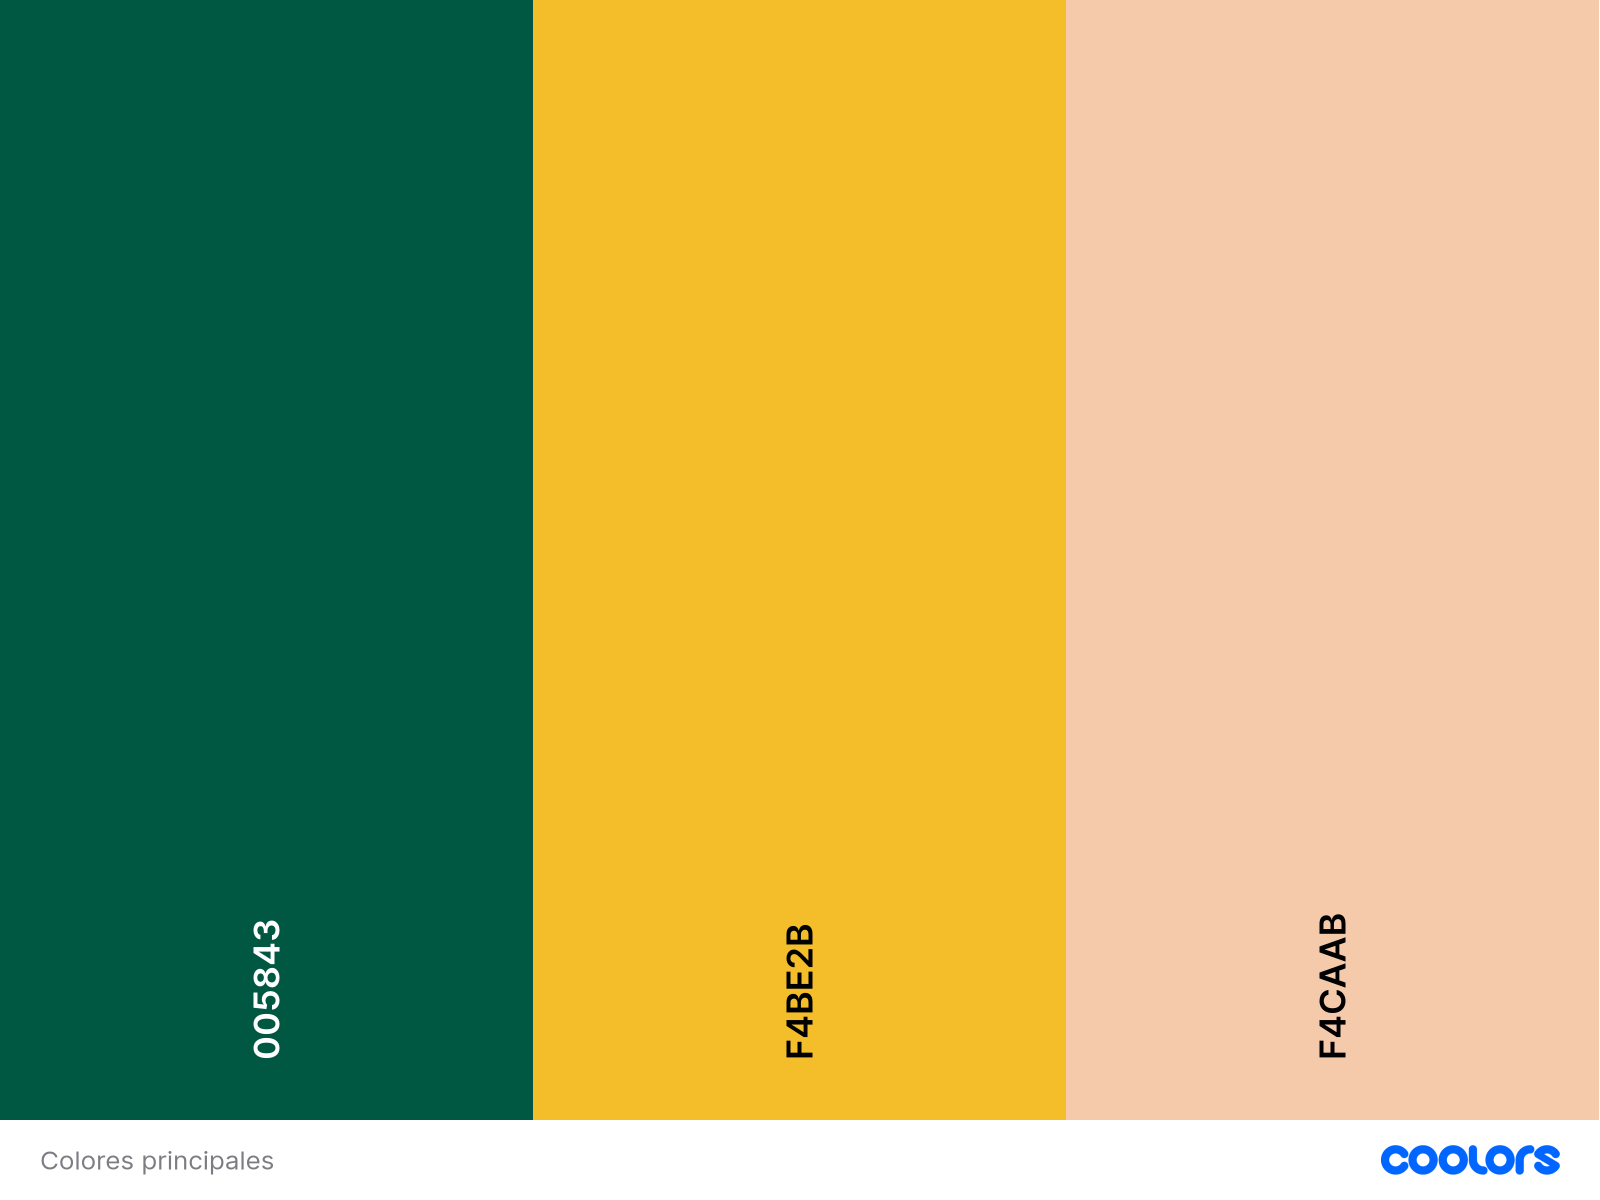
\includegraphics[width=0.66\textwidth]{figures/diseno/colores/Colores principales.png}
                \caption{Colores semilla}
                \label{figure:disenio:colores_semilla}
            \end{figure}
    
            \begin{itemize}
                \item Principal: 
                    \begin{itemize}
                        \item Formato hexadecimal: \#005843
                        \item Formato \gls{hct}: \textit{Hue} 171,954, \textit{Chroma} 34,299 y \textit{Tone} 32,667
                    \end{itemize}
                \item Secundario: 
                    \begin{itemize}
                        \item Formato hexadecimal: \#F4BE2B
                        \item Formato \gls{hct}: \textit{Hue} 87,354, \textit{Chroma} 54,911 y \textit{Tone} 79,747
                    \end{itemize}
                \item Terciario:
                    \begin{itemize}
                        \item Formato hexadecimal: \#F4CAAB
                        \item Formato \gls{hct}: \textit{Hue} 58,088, \textit{Chroma} 18,774 y \textit{Tone} 84,181
                    \end{itemize}
                
            \end{itemize}

            Estos colores principales fueron procesados por \textit{Material Design Builder} generando una serie de variantes, descritas en la Figura \ref{figure:disenio:variantes_colores_principales}. 

            \begin{figure}[h]
                \centering
                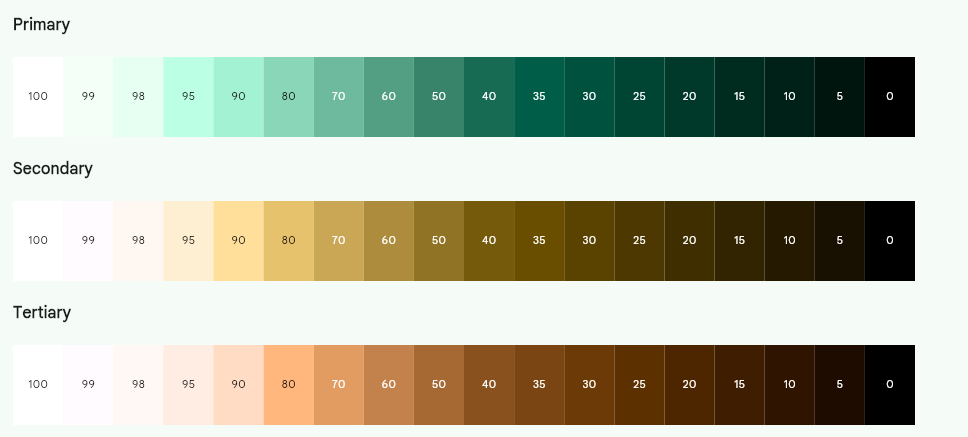
\includegraphics[width=0.8\textwidth]{figures/diseno/colores/Variantes de los colores principales.png}
                \caption{Variantes de los colores principales}
                \label{figure:disenio:variantes_colores_principales}
            \end{figure}

            Con las variantes de esos colores la herramienta genera los colores del modo claro y oscuro; los cuales se pueden ver en las Figuras \ref{figure:disenio:esquema_claro} y \ref{figure:disenio:esquema_oscuro} respectivamente.

            \begin{figure}[h]
                \centering
                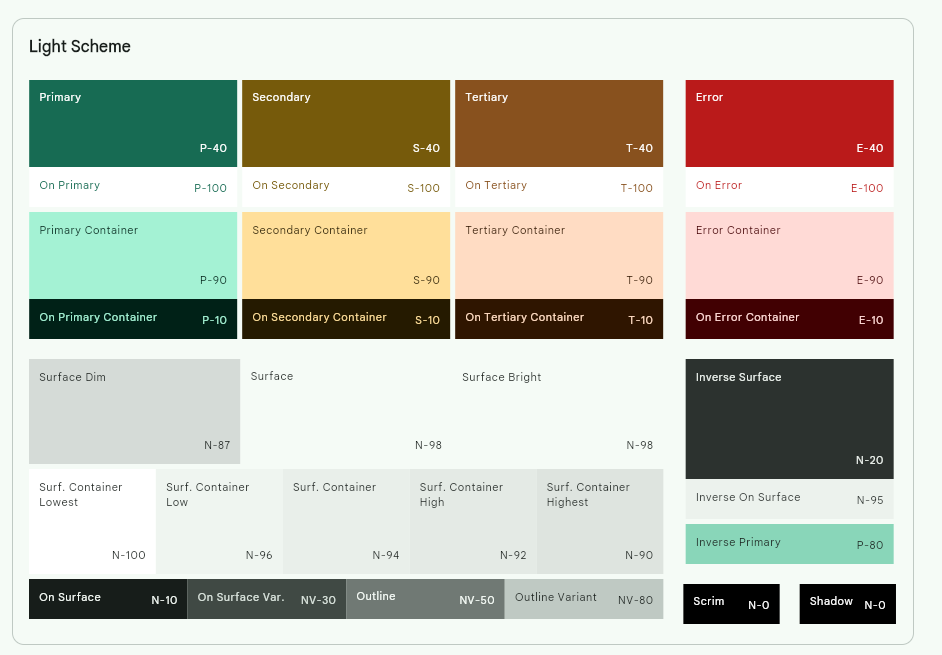
\includegraphics[width=0.8\textwidth]{figures/diseno/colores/Esquema de colores claro.png}
                \caption{Esquema de colores claro}
                \label{figure:disenio:esquema_claro}
            \end{figure}
    
            \begin{figure}[h]
                \centering
                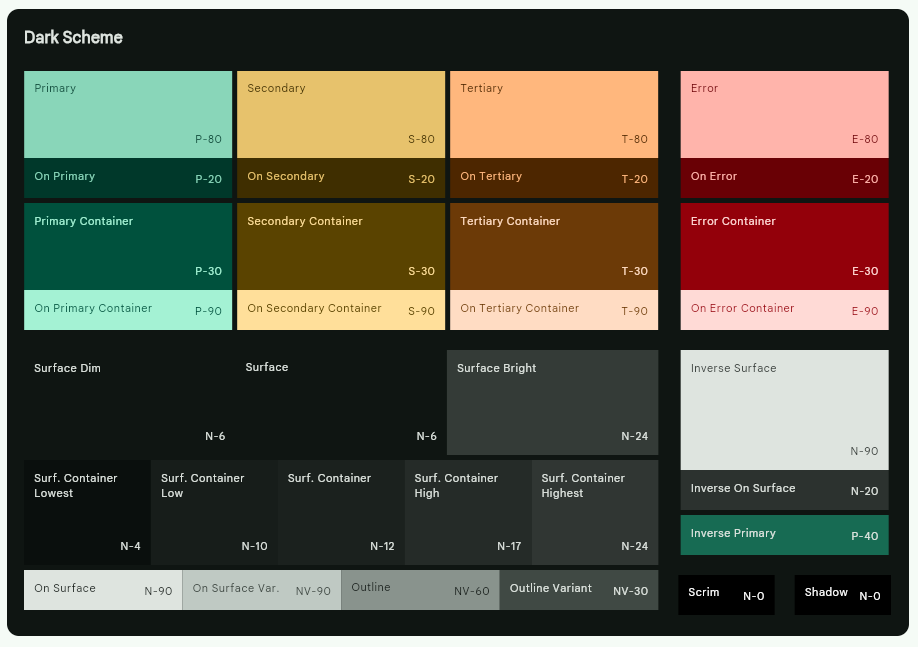
\includegraphics[width=0.8\textwidth]{figures/diseno/colores/Esquema de colores oscuro.png}
                \caption{Esquema de colores oscuro}
                \label{figure:disenio:esquema_oscuro}
            \end{figure}

            En cuanto al logo del sistema, también fue diseñado en colaboración con la asociación \textit{LevelUp}, tomando los colores del mismo de la selección de los colores semilla. En la Figura \ref{figure:disenio:logo} se presenta el icono realizado.

            \begin{figure}[h]
                \centering
                
\includegraphics[width=0.3\textwidth]{figures/diseno/logo.png}
                \caption{Logo del sistema}
                \label{figure:disenio:logo}
            \end{figure}
            
            Asimismo, para convertir el logo a un formato que pudiera utilizarse en Android, se recurrió a la herramienta \href{https://icon.kitchen/}{Icon kitchen}, como se puede visualizar en la Figura \ref{figure:disenio:icon_litchen}.

            \begin{figure}[h]
                \centering
                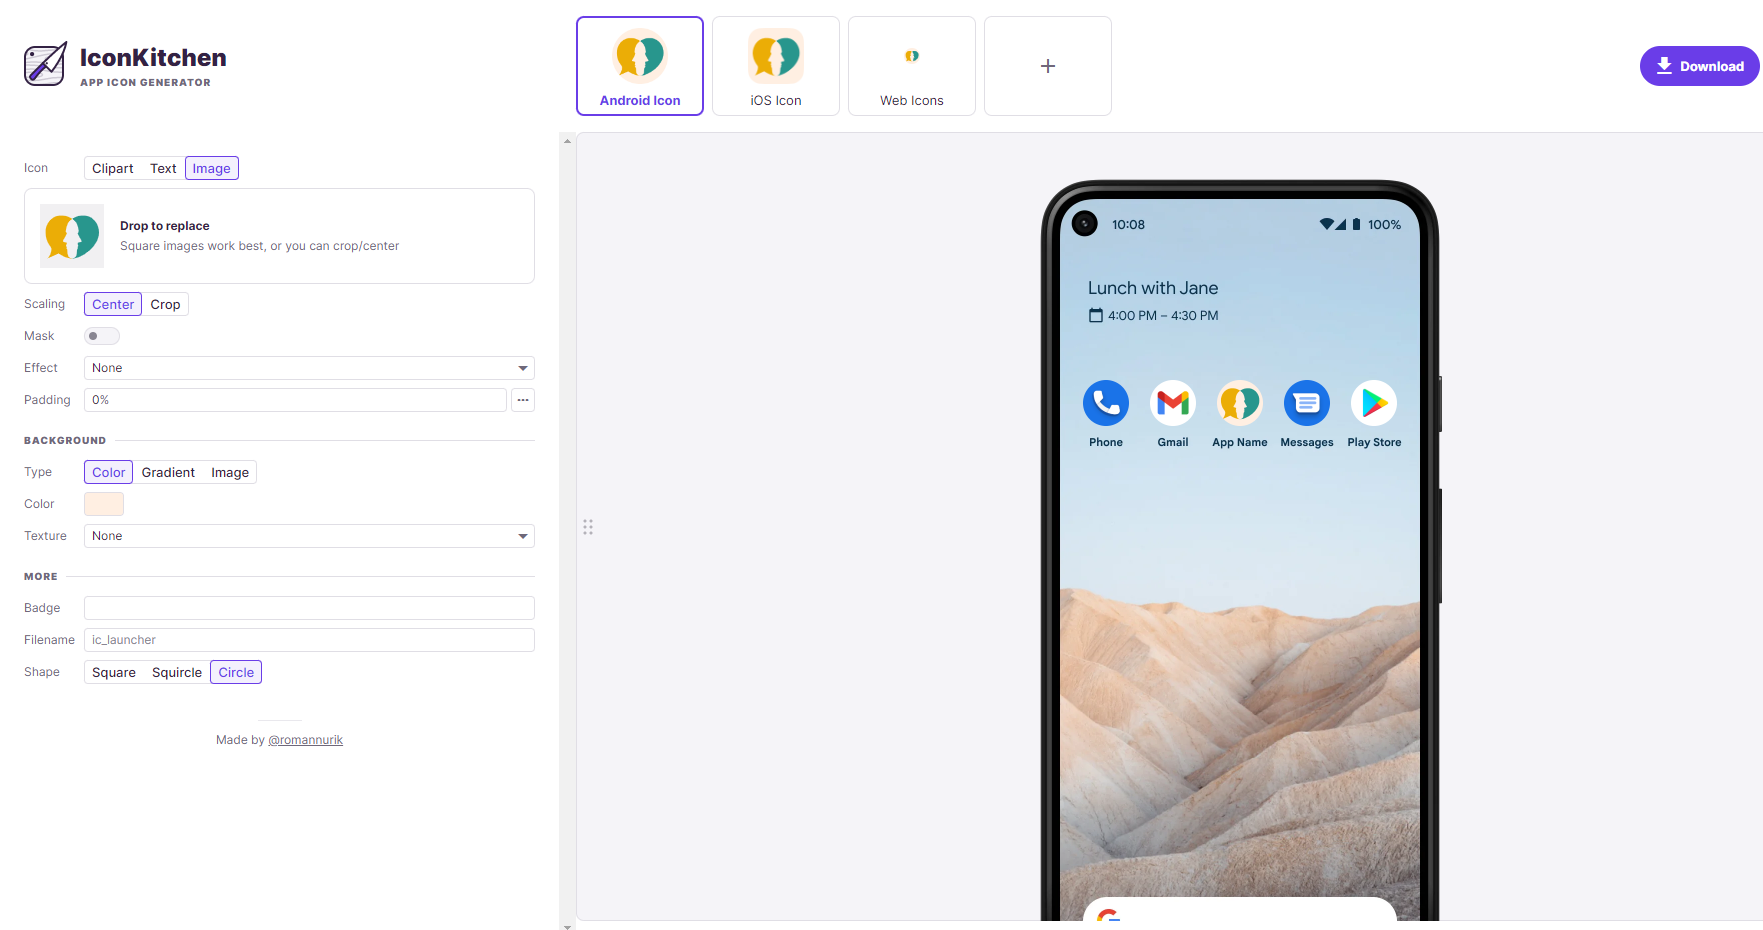
\includegraphics[width=0.66\textwidth]{figures/diseno/Logo icon kitchen.png}
                \caption{Procesado del logo en Icon Kitchen}
                \label{figure:disenio:icon_litchen}
            \end{figure}